\documentclass[11pt]{article}
\usepackage{setspace}
\setstretch{1}
\usepackage{amsmath,amssymb, amsthm}
\usepackage{graphicx}
\usepackage{bm}
\usepackage[hang, flushmargin]{footmisc}
\usepackage[colorlinks=true]{hyperref}
\usepackage[nameinlink]{cleveref}
\usepackage{footnotebackref}
\usepackage{url}
\usepackage{listings}
\usepackage[most]{tcolorbox}
\usepackage{inconsolata}
\usepackage[papersize={8.5in,11in}, margin=1in]{geometry}
\usepackage{float}
\usepackage{caption}
\usepackage{esint}
\usepackage{url}
\usepackage{enumitem}
\usepackage{subfig}
\usepackage{wasysym}
\newcommand{\ilc}{\texttt}
\newcommand{\p}{\partial}
\usepackage{etoolbox}
\usepackage{algorithm}
\usepackage{changepage}
% \usepackage{algorithmic}
\usepackage[noend]{algpseudocode}
\usepackage{tikz}


\usetikzlibrary{matrix,positioning,arrows.meta,arrows}
\patchcmd{\thebibliography}{\section*{\refname}}{}{}{}
% \PassOptionsToPackage{hyphens}{url}\usepackage{hyperref}

\providecommand{\myceil}[1]{\left \lceil #1 \right \rceil }
\providecommand{\myfloor}[1]{\left \lfloor #1 \right \rfloor }

\definecolor{dkgreen}{rgb}{0,0.6,0}
\definecolor{gray}{rgb}{0.5,0.5,0.5}
\definecolor{mauve}{rgb}{0.58,0,0.82}

\lstset{frame=tb,
  language=Python,
  aboveskip=3mm,
  belowskip=3mm,
  showstringspaces=false,
  columns=flexible,
  basicstyle={\small\ttfamily},
  numbers=none,
  numberstyle=\tiny\color{gray},
  keywordstyle=\color{blue},
  commentstyle=\color{dkgreen},
  stringstyle=\color{mauve},
  breaklines=true,
  breakatwhitespace=true,
  tabsize=3
}

\begin{document}


\title{\textbf{CSDS 491: Assignment 3}}

\author{Shaochen (Henry) ZHONG, \ilc{sxz517@case.edu}}

\date{Due and submitted on 03/29/2021 \\ Spring 2021, Dr. Lewicki}
\maketitle


% We've received some common questions for A1.  Here are some hints to help you go in the right direction.
%
% Q2.2: You need only prove there is a logical gap that would require an additional assumption.
%
% Q4: It is helpful to use the conjugate prior as shown in lecture.  The  normalization factor for the posterior then has the same form as the prior (but with different arguments).
%
% Q5: Remember that the data consists of event times, and the posterior is in terms of the Poisson rate parameter lambda given the number of observed data events in a given duration from 0 to T.  You only need a single Poisson likelihood combined with the prior to get the posterior.
%
% Exploration: The terms discrete and continuous refer to the variables in the model.  See the rubric for the grading criteria. Try to make your inference problems simple models of real-world situations, rather than just numerical examples.


\section*{E1. MRFs and Images Denoising}

\subsection*{1.1.}

Per question, known that the total energy of the system is:

\begin{equation*}
    E(x, y) = h \sum_{i} x_i - \beta \sum_i \sum_{j \in ne(x_i)} x_i x_j - \eta \sum_i x_i y_i
\end{equation*}

By ``letting out'' $x_k$, we have the following:

\begin{align*}
    E(x, y) &= (h \sum_{i / k} x_i - \beta \sum_{i / k} \sum_{j \in ne(x_i) / k} x_i x_j - \eta \sum_{i / k} x_i y_i) + h \cdot x_k - \beta \sum_{j \in ne(x_k) }x_k x_j - \beta \sum_{j \in ne(x_k) } x_j x_k- \eta x_k y_k \\
    &= C + h \cdot x_k - \beta \sum_{j \in ne(x_k) }x_k x_j - \beta \sum_{j \in ne(x_k)}  x_j x_k- \eta x_k y_k
\end{align*}

On the other hand, assume $x$ is now $\overline{x}$ with $x_k$ flipped, we must have:

\begin{align*}
    E(\overline{x}, y) &= (h \sum_{i / k} x_i - \beta \sum_{i / k} \sum_{j \in ne(x_i) / k} x_i x_j - \eta \sum_{i / k} x_i y_i) + h \cdot x_k - \beta \sum_{j \in ne(x_k) }x_k x_j - \beta \sum_{j \in ne(x_k) } x_j x_k- \eta x_k y_k \\
    &= C + h \cdot (-x_k) - \beta \sum_{j \in ne(x_k)} (-x_k) x_j - \beta \sum_{j \in ne(x_k) }x_j (-x_k) - \eta (-x_k) y_k
\end{align*}

Thus, the change in energy will be:

\begin{align*}
    \Delta E &= E(\overline{x}, y) - E(x, y) \\
    &= C - C -2 h \cdot x_k -4\beta \sum_{j \in ne(x_k)} (-x_k) x_j + 2 \eta x_k y_k \\
    &= -2 h \cdot x_k + 4\beta \sum_{j \in ne(x_k)} x_k x_j + 2 \eta x_k y_k
\end{align*}



\subsection*{1.2.}

You may refer to \ilc{A3/code/e1.py} for my code, the method for energy updating calculation is \ilc{denoise()}. Currently my method is ``updated'' for tasks of below questions so it might be a little complicate to read, but the generally idea is to:

\begin{itemize}
    \item Pick one pixel
    \item Calculate the energy change $\Delta E$ in terms of first (with parameter $h$), second (with parameter $\beta$), and third (with parameter $\eta$) terms per each pixel.
    \item Check if the energy change $\Delta E$ is negative, if so, flip the pixel. This is because lower energy yields a higher probablity $p(x, y)$, so the pixel-just-flipped is more likely to be a noise pixel.
    \item Proceed to the next pixel. In my case I just loop through every pixel along their indicies.
\end{itemize}

\subsection*{1.3.}

\begin{figure}[H]
    \centering
    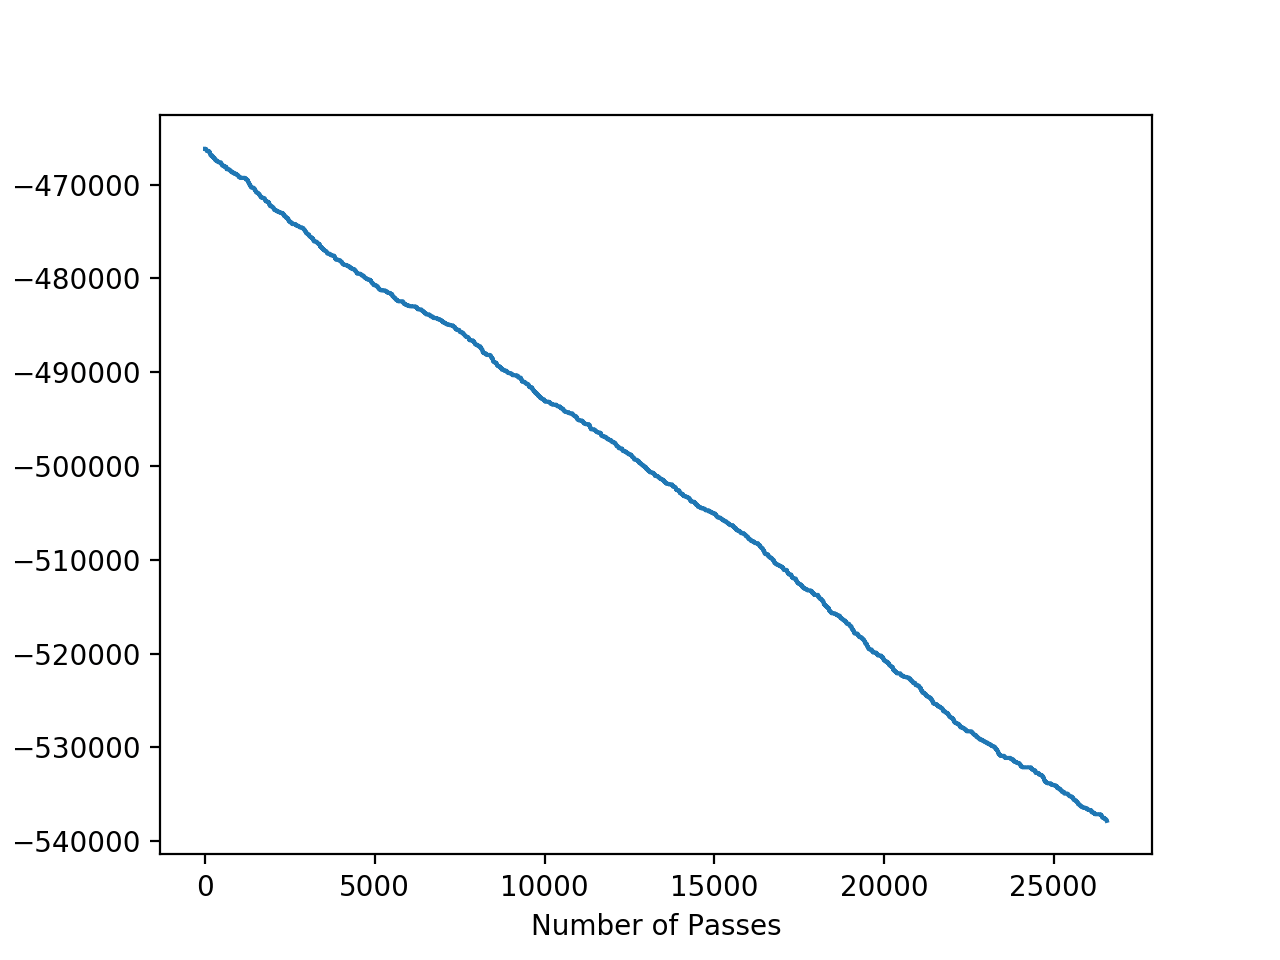
\includegraphics[width=0.5\linewidth]{{fig/E1.3}.png}
\end{figure}
As whenever the $\Delta E$ is negative, we take the flip, the overall energy is decreasing through out the whole process as the passing number increasing.

\subsection*{1.4.}


\begin{figure}[H]
\minipage{0.25\textwidth}
  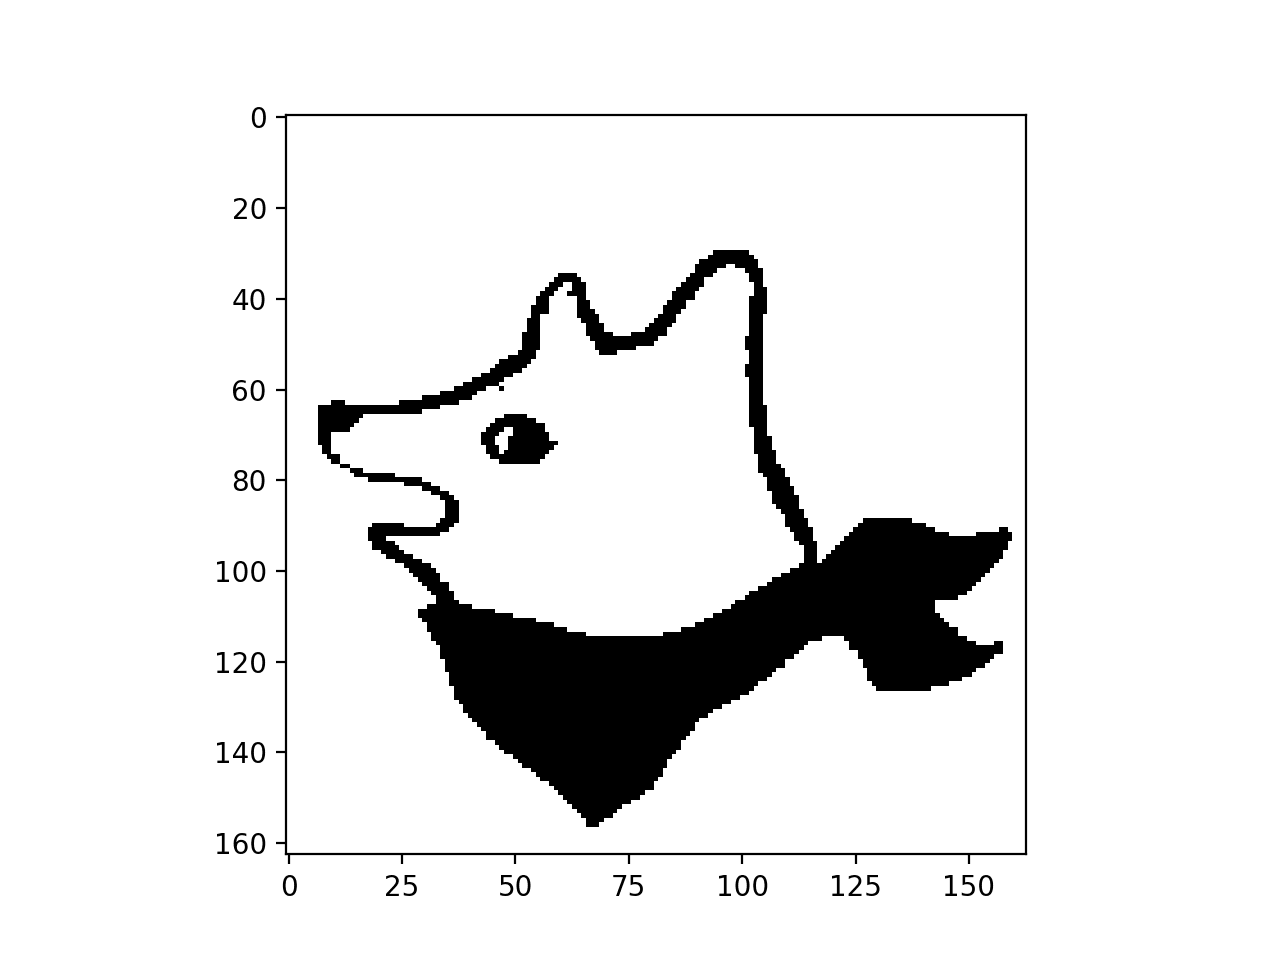
\includegraphics[width=\linewidth]{{fig/E1.4}.png}
  \caption*{Original Image}
\endminipage\hfill
\minipage{0.25\textwidth}
    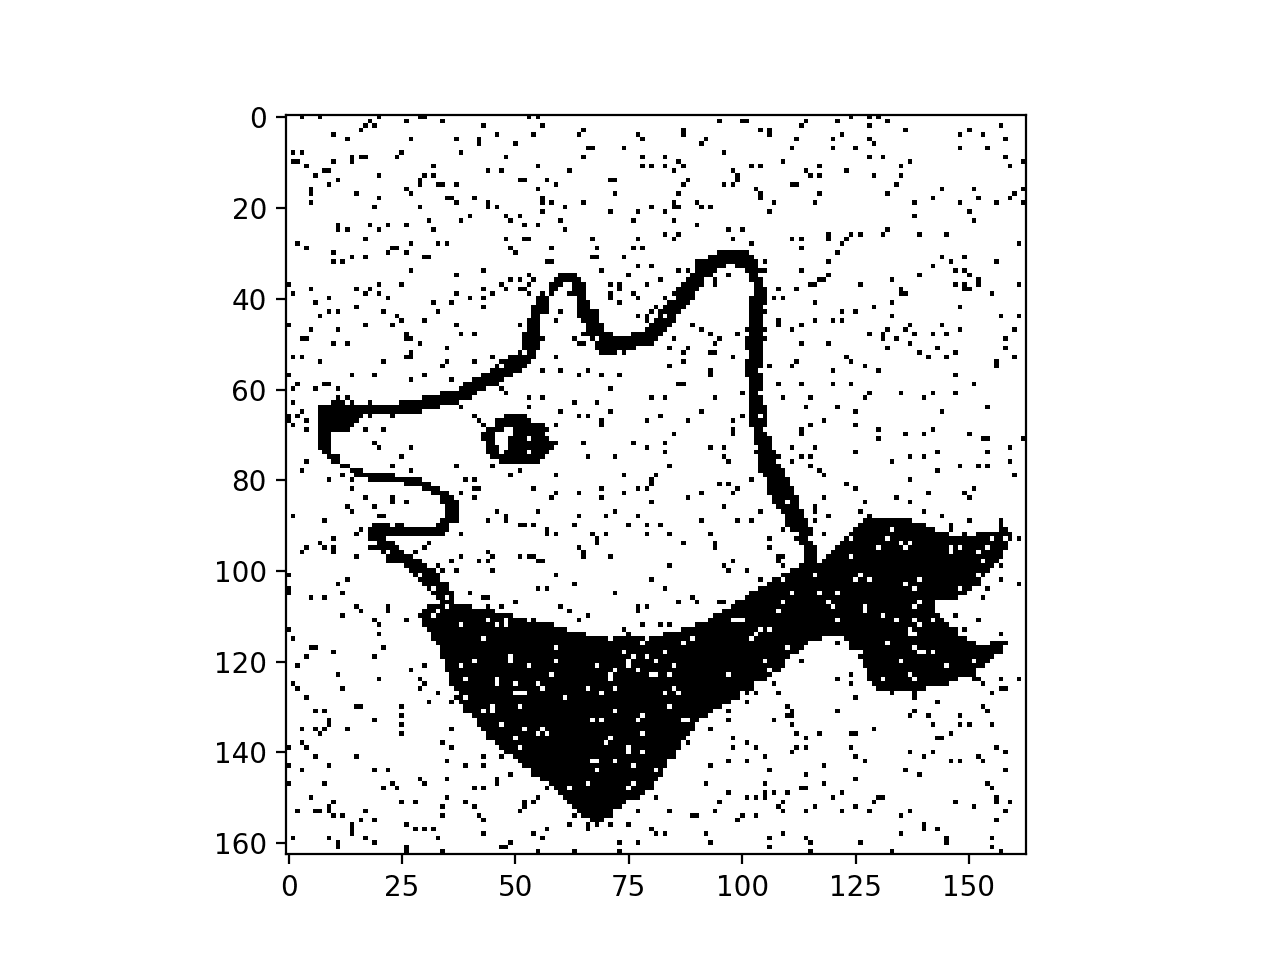
\includegraphics[width=\linewidth]{{fig/E1.4.1}.png}
    \caption*{Noised Image}
\endminipage\hfill
\minipage{0.25\textwidth}
    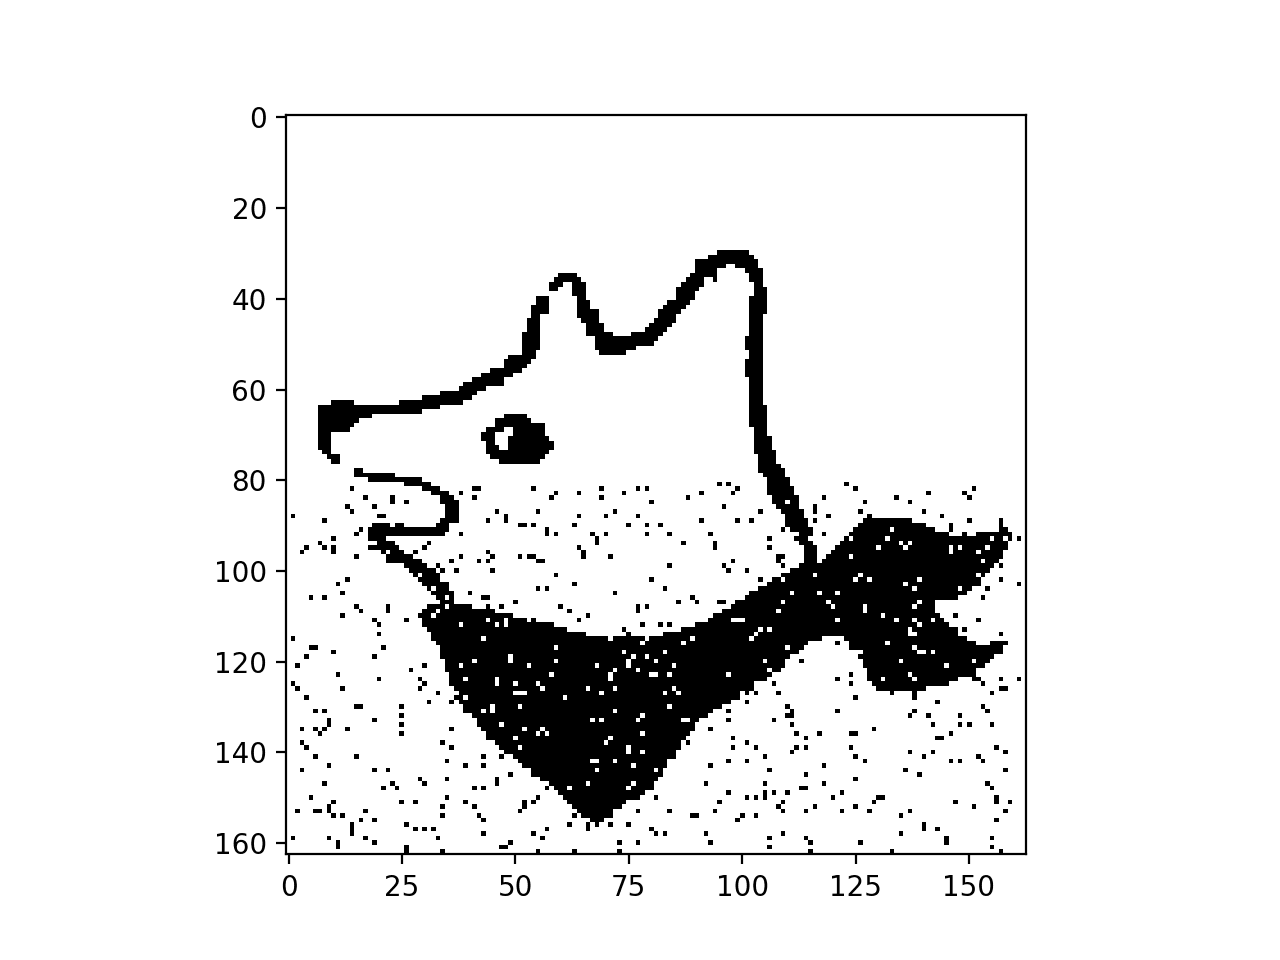
\includegraphics[width=\linewidth]{{fig/E1.4.2}.png}
    \caption*{50\% Denoised}
\endminipage\hfill
\minipage{0.25\textwidth}
    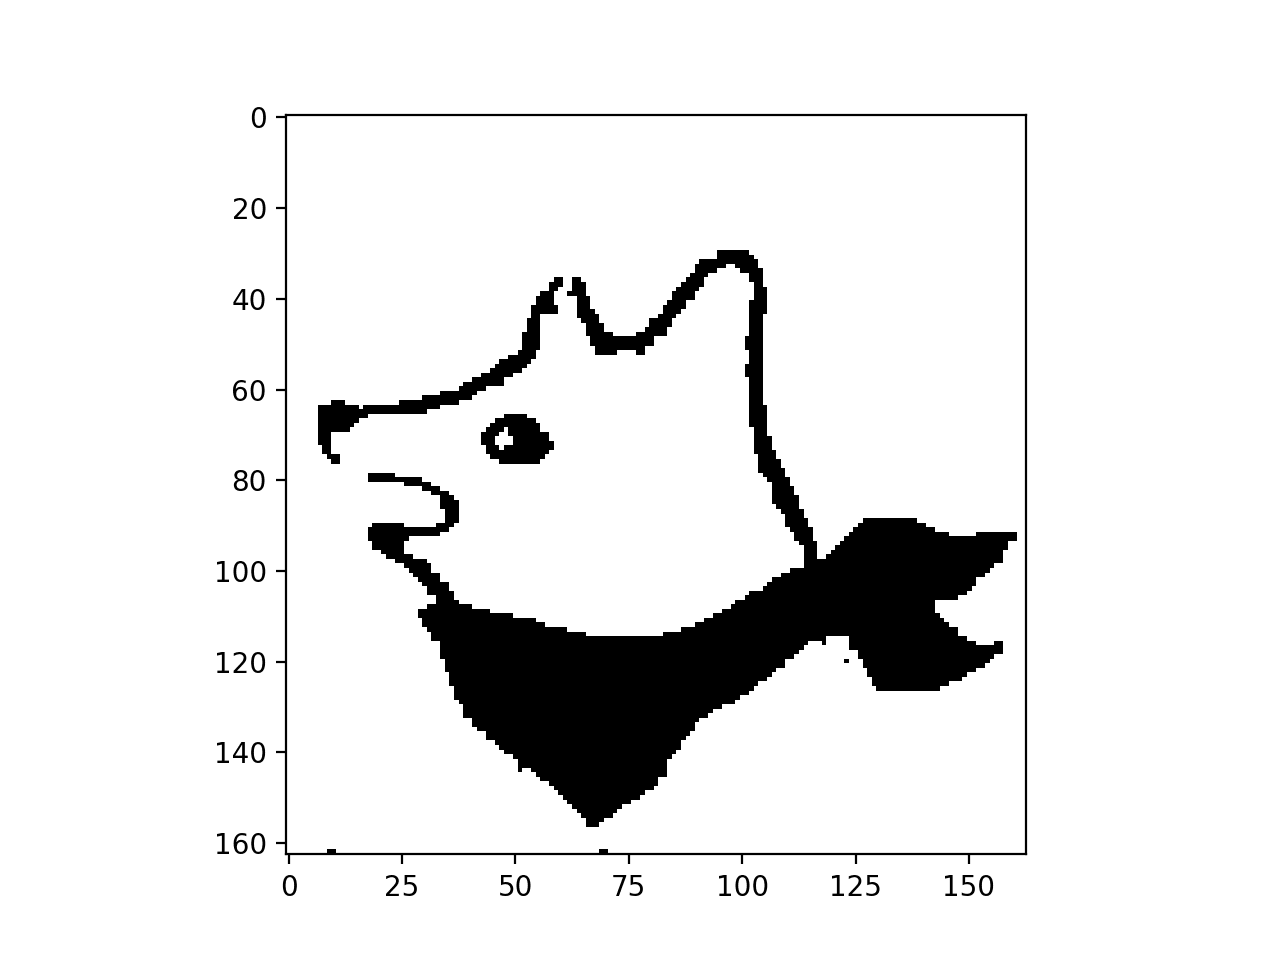
\includegraphics[width=\linewidth]{{fig/E1.4.3}.png}
    \caption*{Fully Denoised}
\endminipage
\end{figure}

Note since I iterate through all pixels along their indicies, so the 50\% image seems only ``top half denoised.'' If I use random order evaluate all pixels, there won't be such distinction.


\subsection*{1.5.}

So we have three paramaters to evaluate. The $h$ is regarding the original value of pixel-in-question, the $\beta$ is regarding the neighbors of the pixel-in-question, and the $\eta$ is about the change of pixel-in-question (if flipped, energy decrease, otherwise increase).

It is my understanding that $h$ serves as a bias of the model, where as it prefer a pixel value more than the other. In the case that $h > 0$, the model will prefer pixels with $1$-value (white); and if $h < 0$, the model will prefer pixel with $-1$-value (black). We may confirm this theory by comparing the following trials:


\begin{figure}[H]
\minipage{0.25\textwidth}
  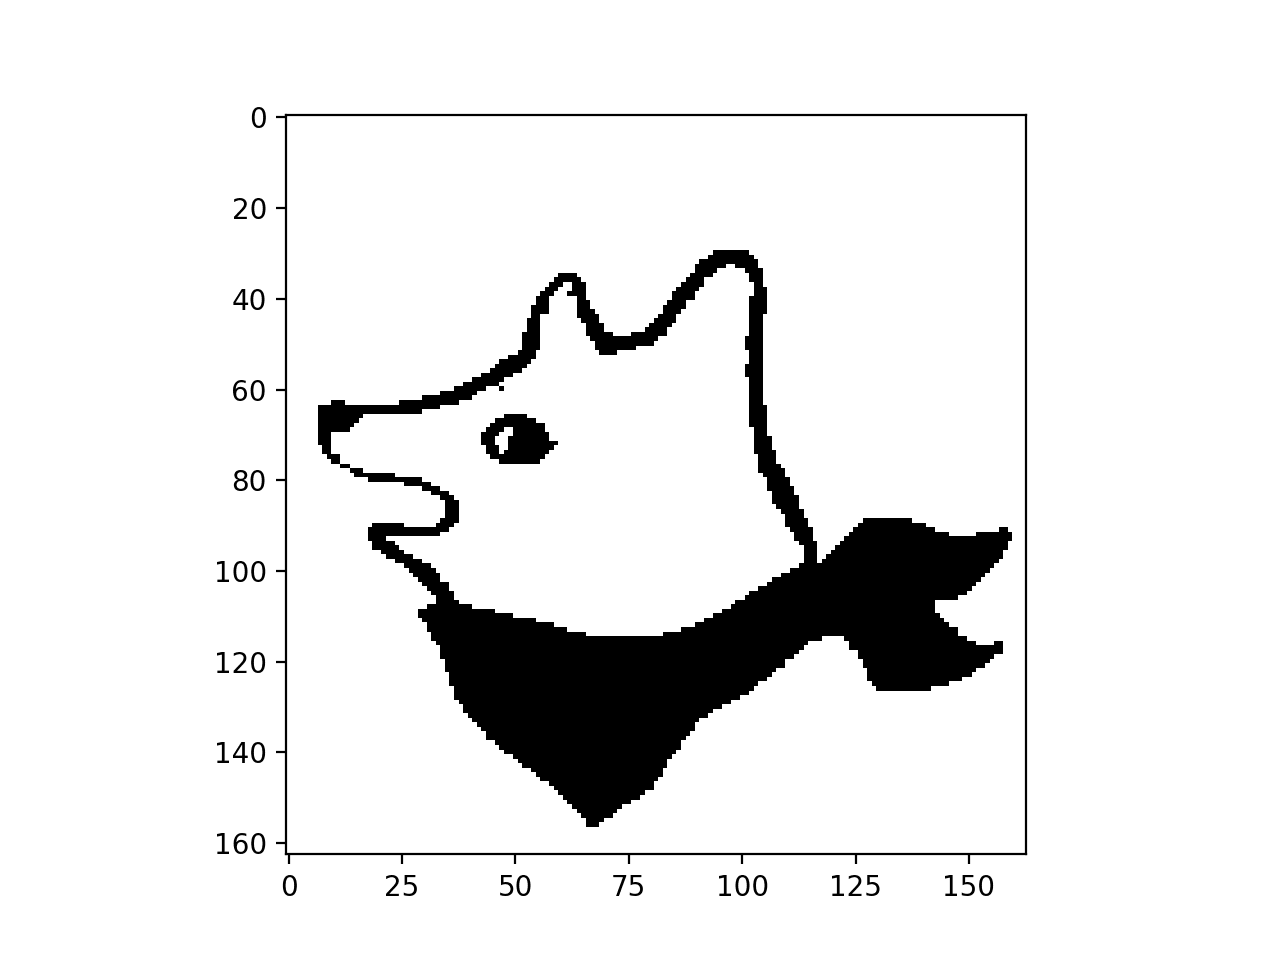
\includegraphics[width=\linewidth]{{fig/E1.4}.png}
  \caption*{Original Image}
\endminipage\hfill
\minipage{0.25\textwidth}
    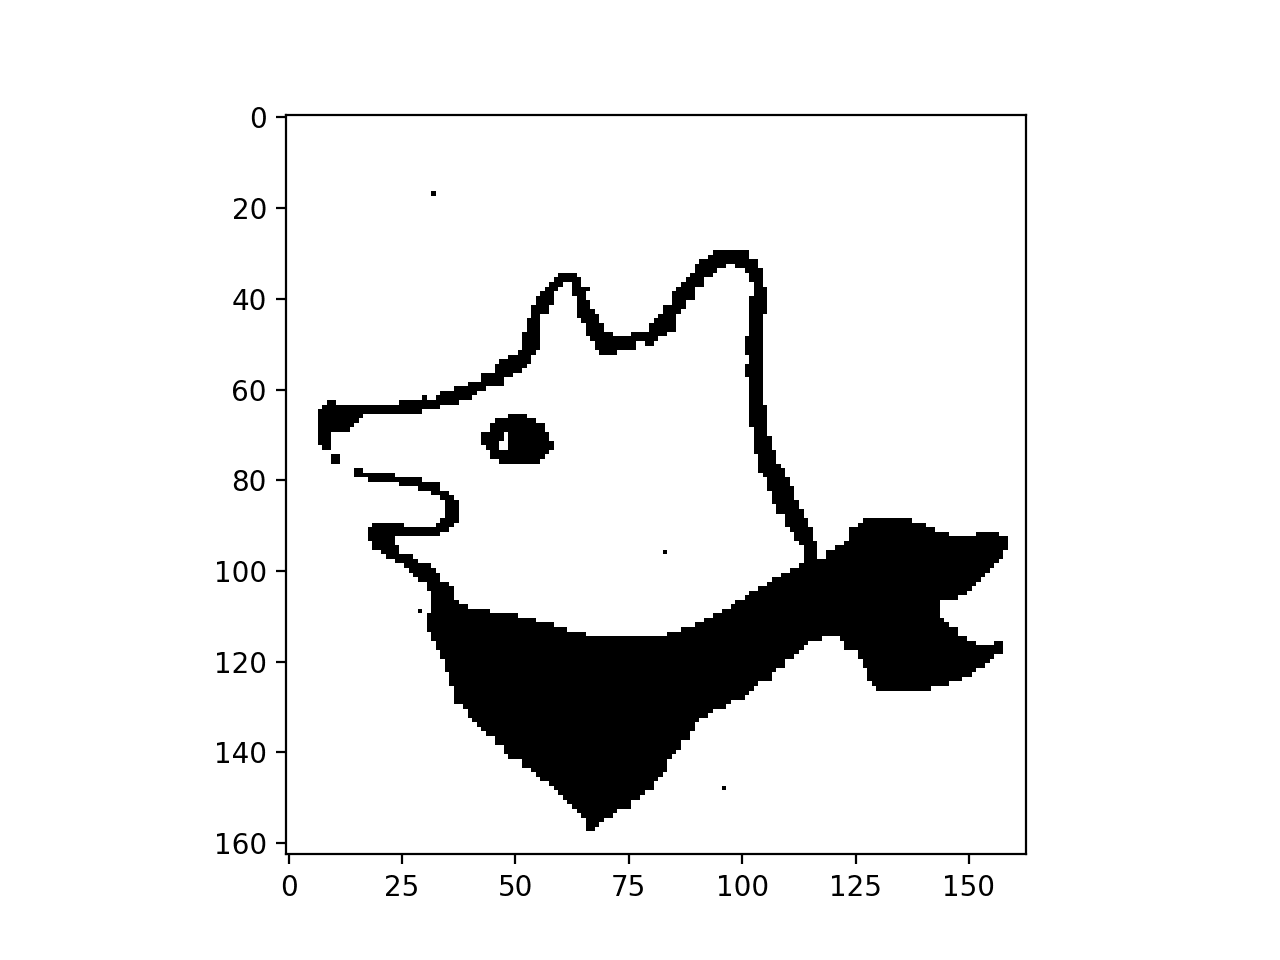
\includegraphics[width=\linewidth]{{fig/E1.5.1}.png}
    \caption*{$h = -2, \beta = 2, \eta = 2$}
\endminipage\hfill
\minipage{0.25\textwidth}
    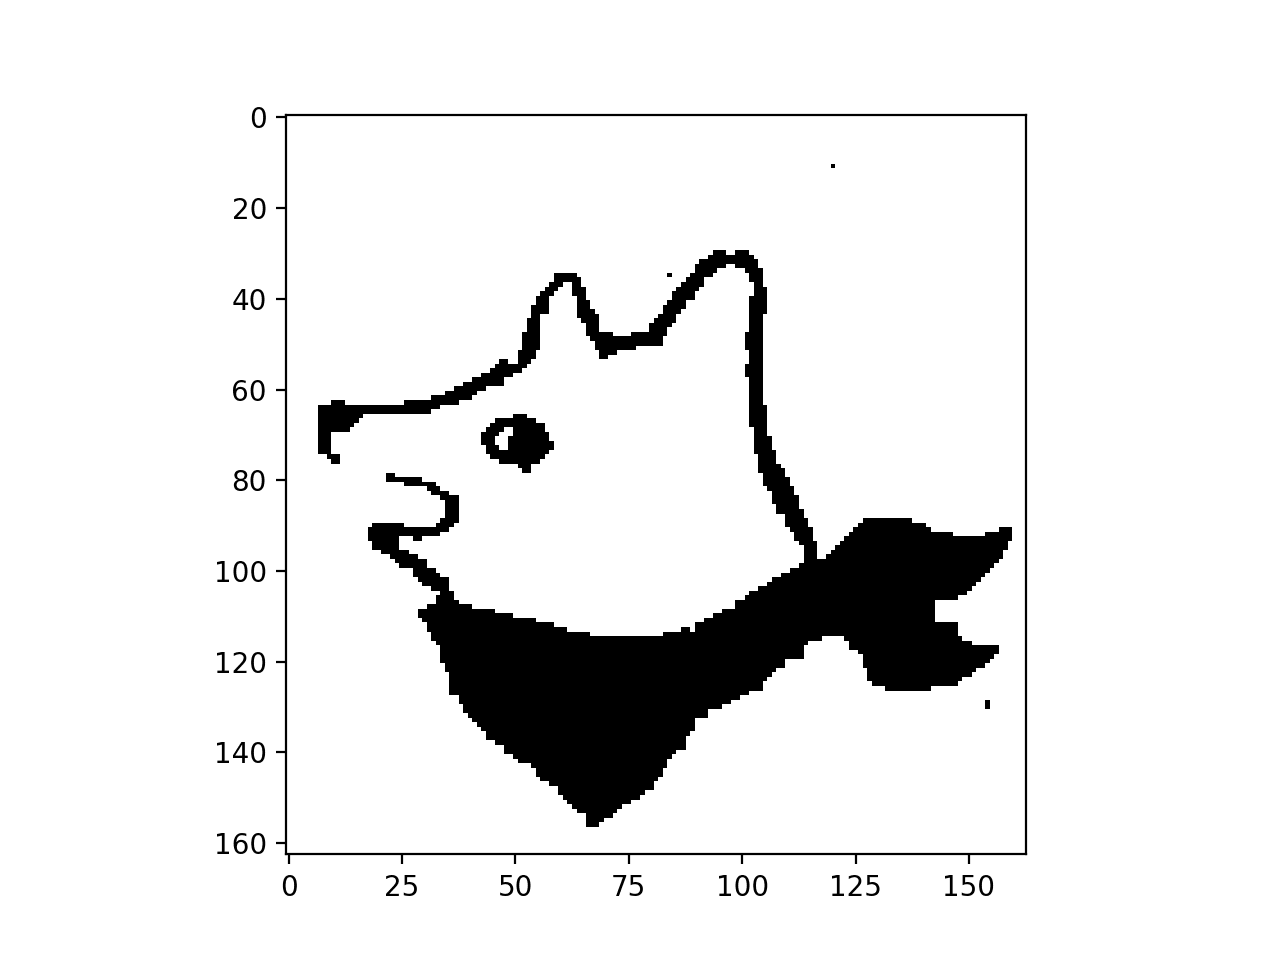
\includegraphics[width=\linewidth]{{fig/E1.5.2}.png}
    \caption*{$h = 2, \beta = 2, \eta = 2$}
\endminipage
\end{figure}

where the $h>0$ result contains more white pixels to $h<0$ trial.\newline

\noindent The $\beta$ term is about the neighbors of a pixel. With $\beta$ being larger, the resultant picture will look more ``clustered'' pixel nearby will tend to be the same color.

\begin{figure}[H]
\minipage{0.25\textwidth}
  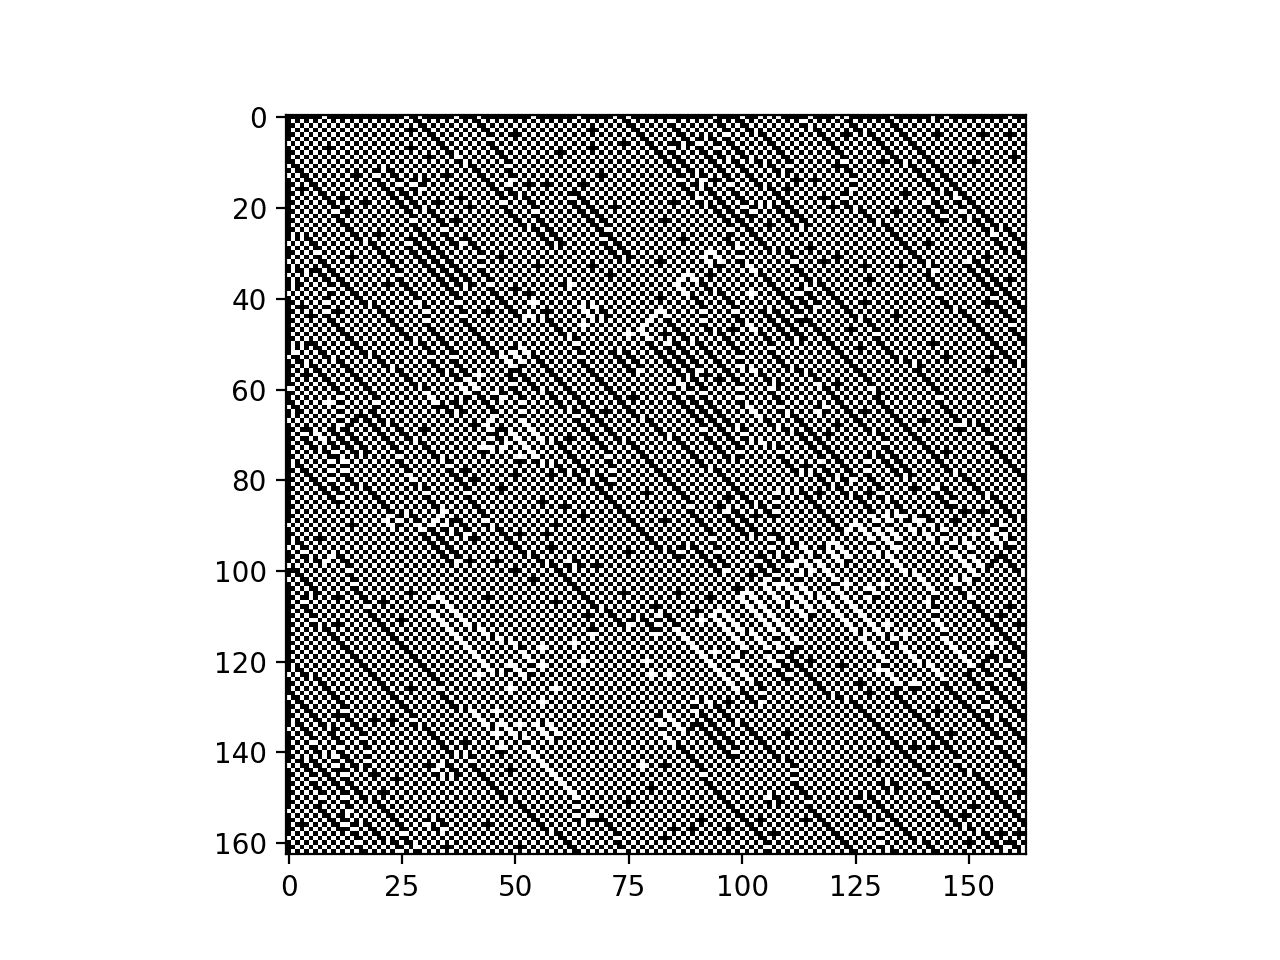
\includegraphics[width=\linewidth]{{fig/E1.5.3}.png}
  \caption*{$h = 0, \beta = -2, \eta = 2$}
\endminipage\hfill
\minipage{0.25\textwidth}
    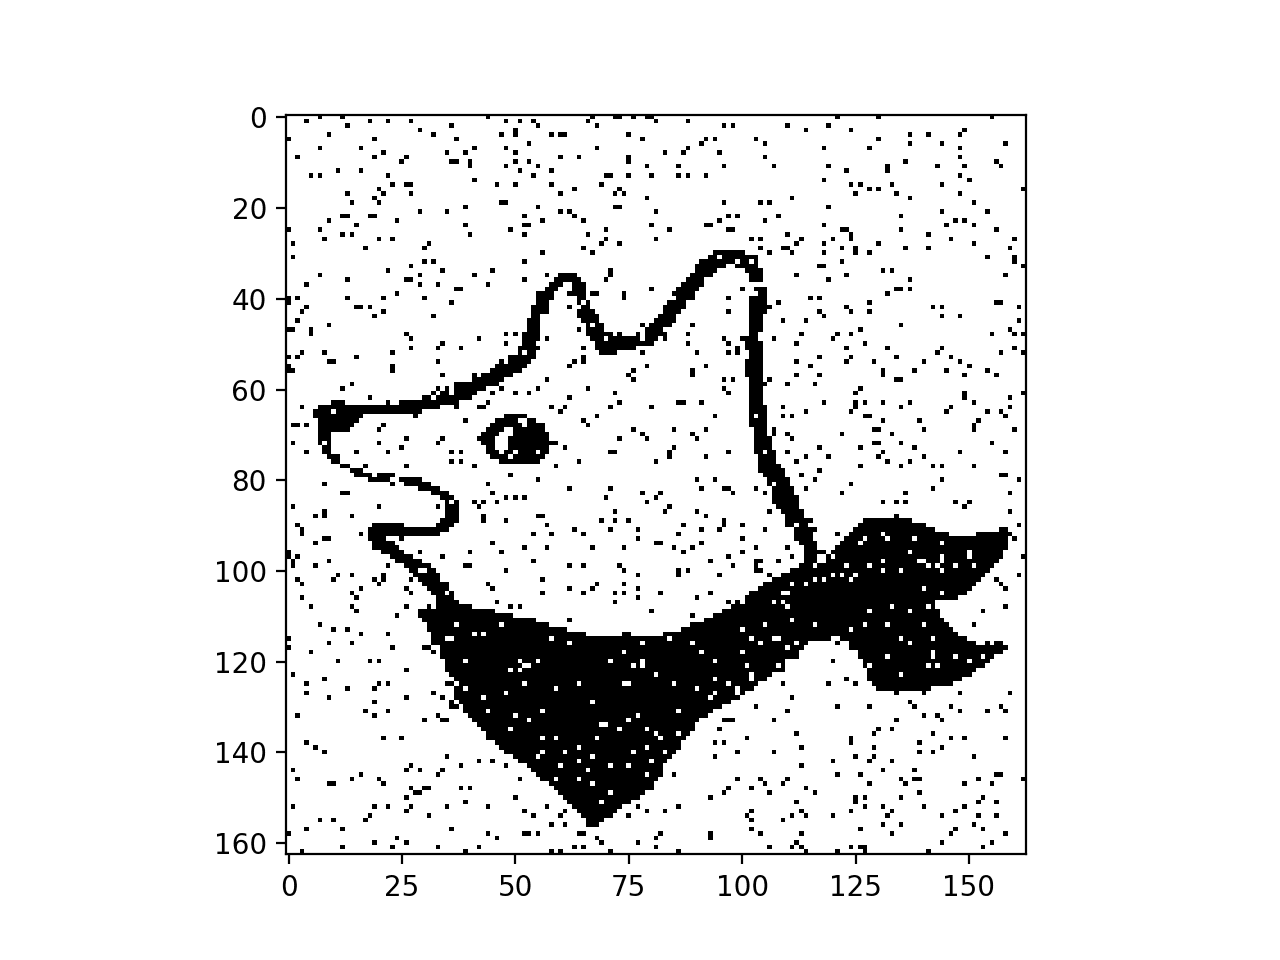
\includegraphics[width=\linewidth]{{fig/E1.5.4}.png}
    \caption*{$h = 0, \beta = 0, \eta = 2$}
\endminipage\hfill
\minipage{0.25\textwidth}
    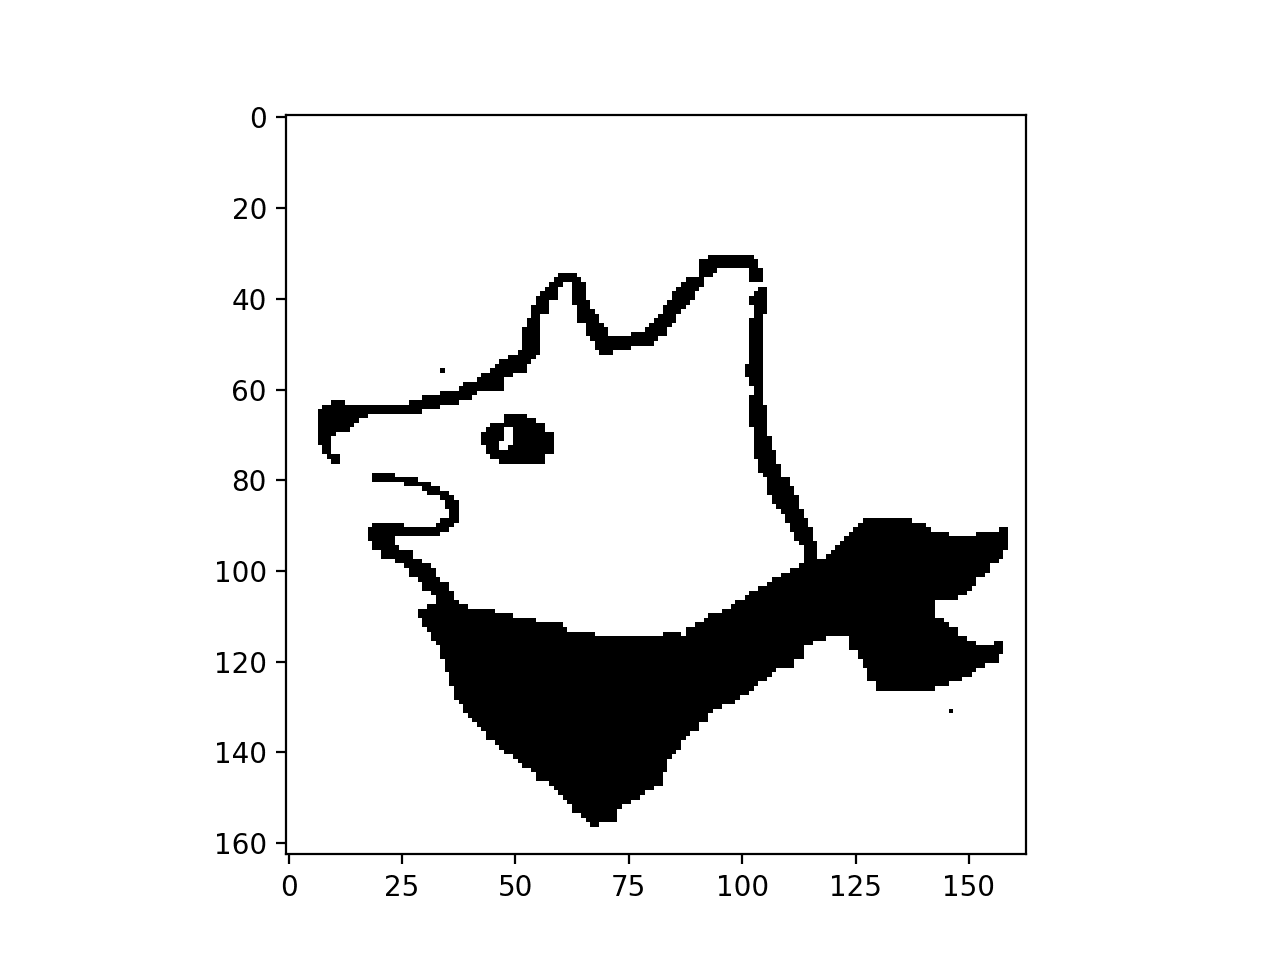
\includegraphics[width=\linewidth]{{fig/E1.5.5}.png}
    \caption*{$h = 0, \beta = 2, \eta = 2$}
\endminipage
\end{figure}

It is clear that with $\beta < 0$, the model tend to believe there's no consistancy between nearby pixels and therefore more ``noisy''. With $\beta = 0$ and no $h$ bias, since there is no flip of pixel (and thus no $\eta$ term decrease), the model will not conduct any denoise operation. With $\beta > 0$, we have a meaning denoised result as expected.\newline


\noindent Last, the $\eta$ term represent the relationship between the noised image and the original image. As we perviously mentioned, such term will decrese if a flip occurs and increase if the value is kept; so a large $\eta$ will encourage the model to kept the pixel value of the noised image. This is probably only good if the original image has minimum amount of noise added.


\begin{figure}[H]
\minipage{0.25\textwidth}
  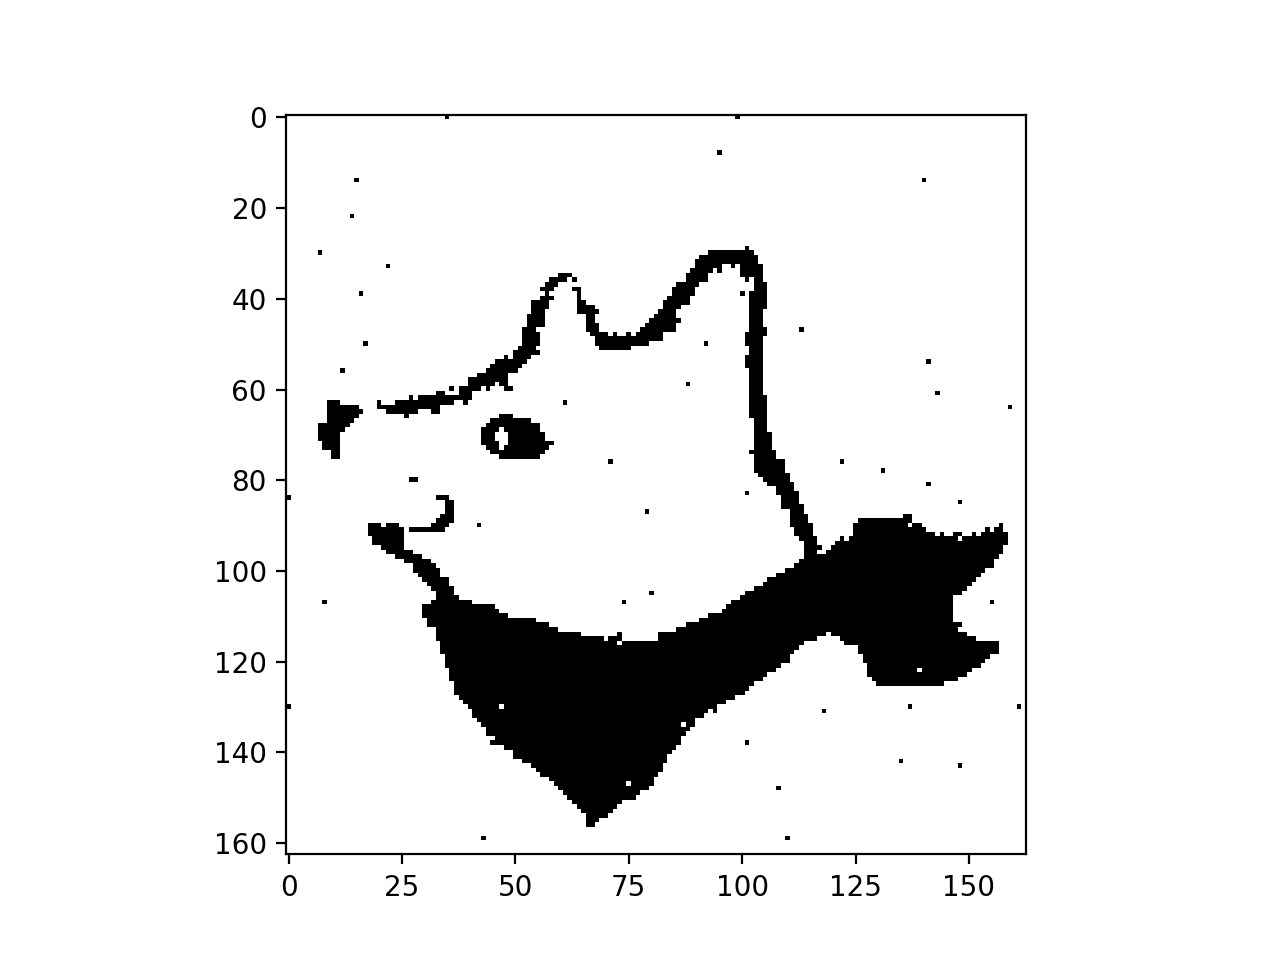
\includegraphics[width=\linewidth]{{fig/E1.5.6}.png}
  \caption*{$h = 0, \beta = 2, \eta = -2$}
\endminipage\hfill
\minipage{0.25\textwidth}
    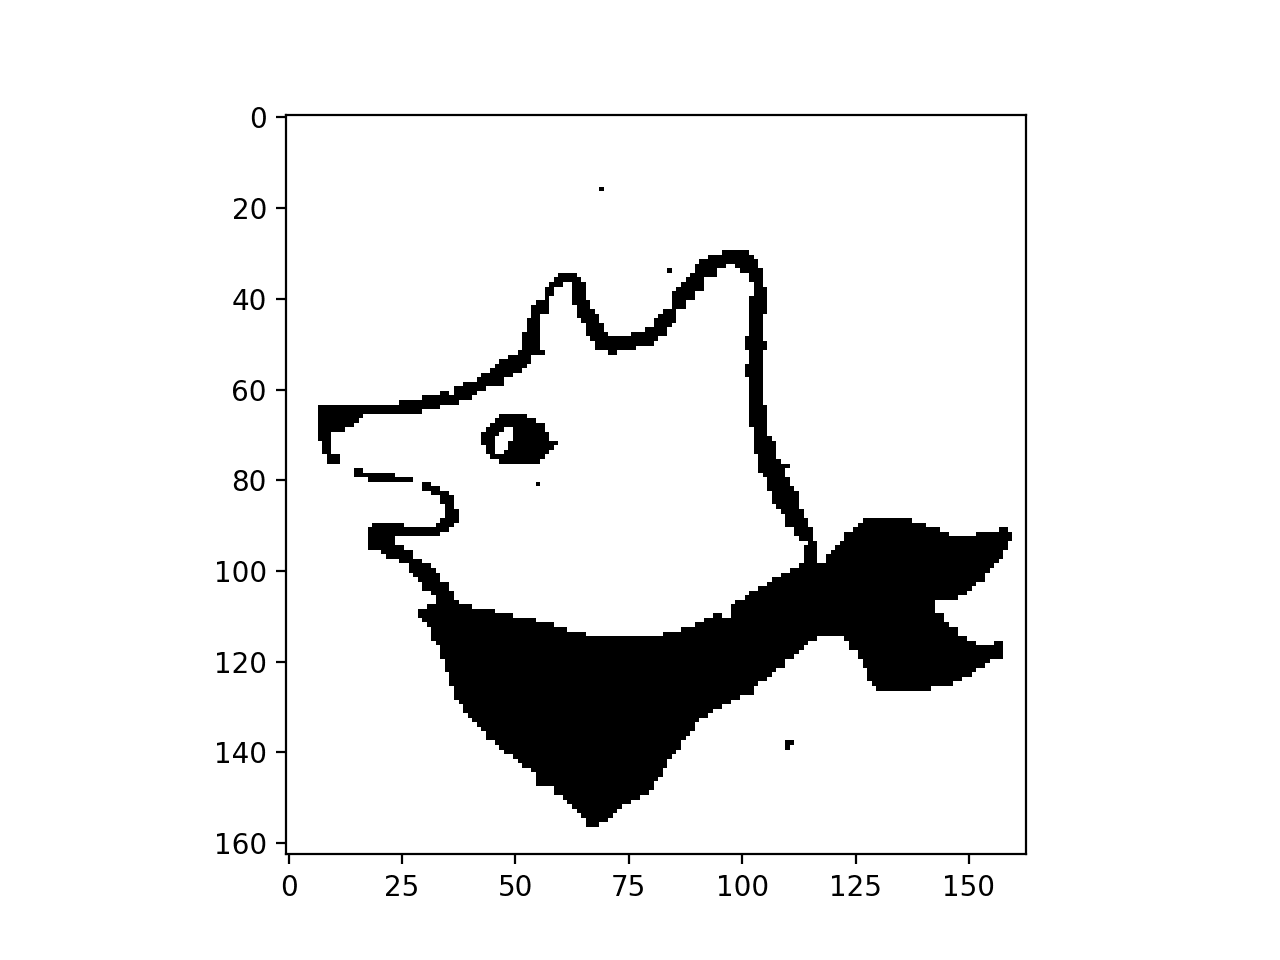
\includegraphics[width=\linewidth]{{fig/E1.5.7}.png}
    \caption*{$h = 0, \beta = 2, \eta = 0$}
\endminipage\hfill
\minipage{0.25\textwidth}
    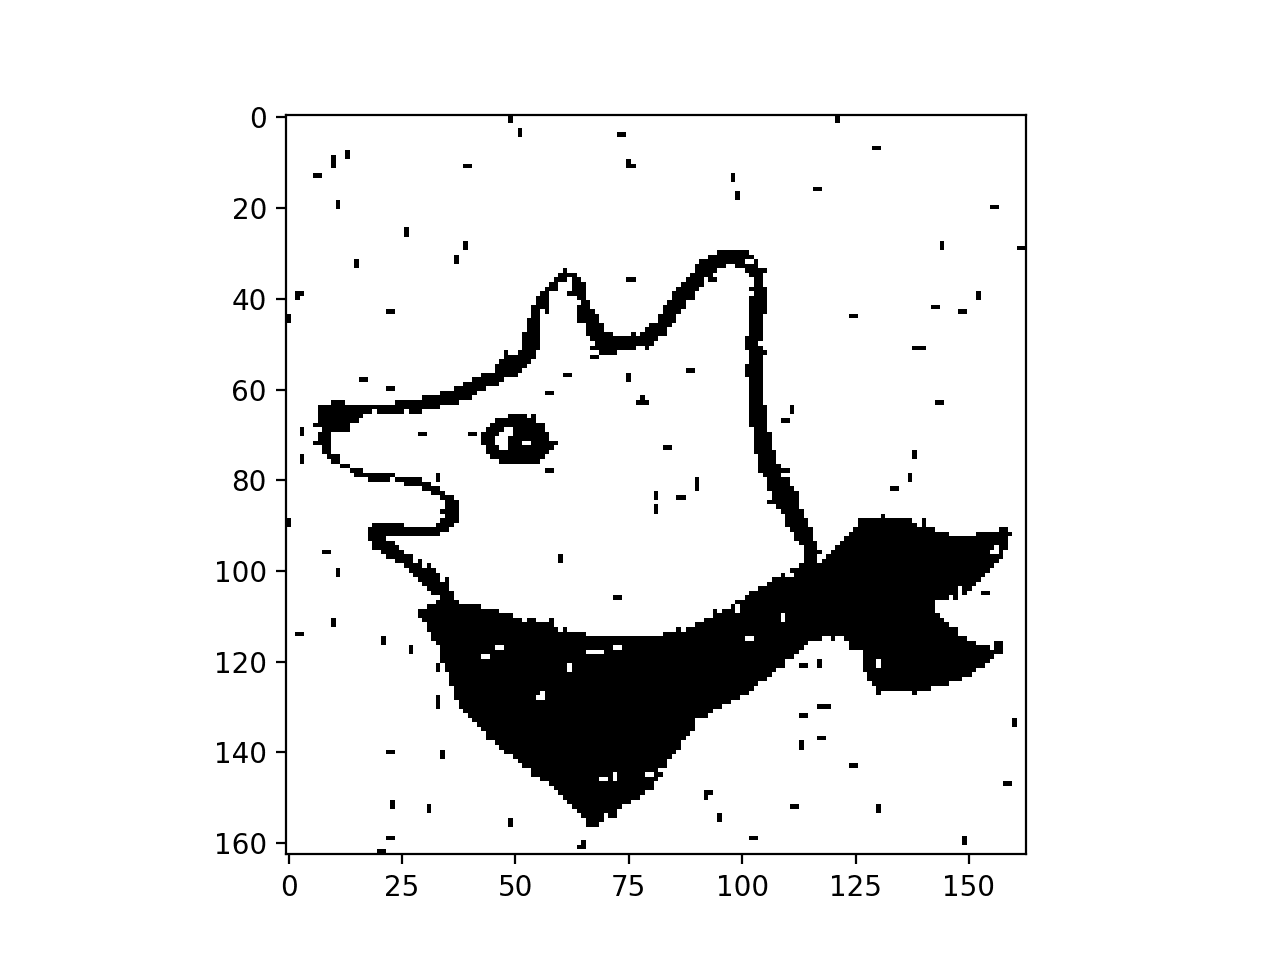
\includegraphics[width=\linewidth]{{fig/E1.5.8}.png}
    \caption*{$h = 0, \beta = 2, \eta = 10$}
\endminipage
\end{figure}

We may observe that with $\eta < 0$, flipping is encouraged so a lot of information became missing. As $\eta$ increase, the model became reluctant to flip and therefore many noisy pixels remain.

\subsection*{1.6.}

I'd like my new energy function to not only consider the four direct neighbors of the pixel-in-question, but also its four other ``corner neighbors.'' On top of this, I'd like each pixel-in-question to expand one extra ``layer'' of scoupe when evaluting neighbors, as it will take the more distant neighbor of neighbors into consideration.

\begin{align*}
    E(x, y) = h \sum_{i} x_i - \beta \sum_i \sum_{j \in around(x_i)} x_i x_j - \beta \sum_i \sum_{k \in outer(i)} x_i x_k - \eta \sum_i x_i y_i \\
    \Delta E = -2 h \cdot x_k + 4\beta \sum_{j \in around(x_k)} x_k x_j + 4\beta  \sum_i \sum_{k \in outer(i)} x_i x_k + 2 \eta x_k y_k
\end{align*}

Since the original energy function only consider four of the neighbors, it has the potential of offering less desired performances with images of interlaced patterns. This is because the model will only exam the four closest neighbors of each pixel; with images with interlaced patterns it might have trouble of distinguishing actual information verses a large grain noise.

\begin{figure}[H]
\minipage{0.25\textwidth}
  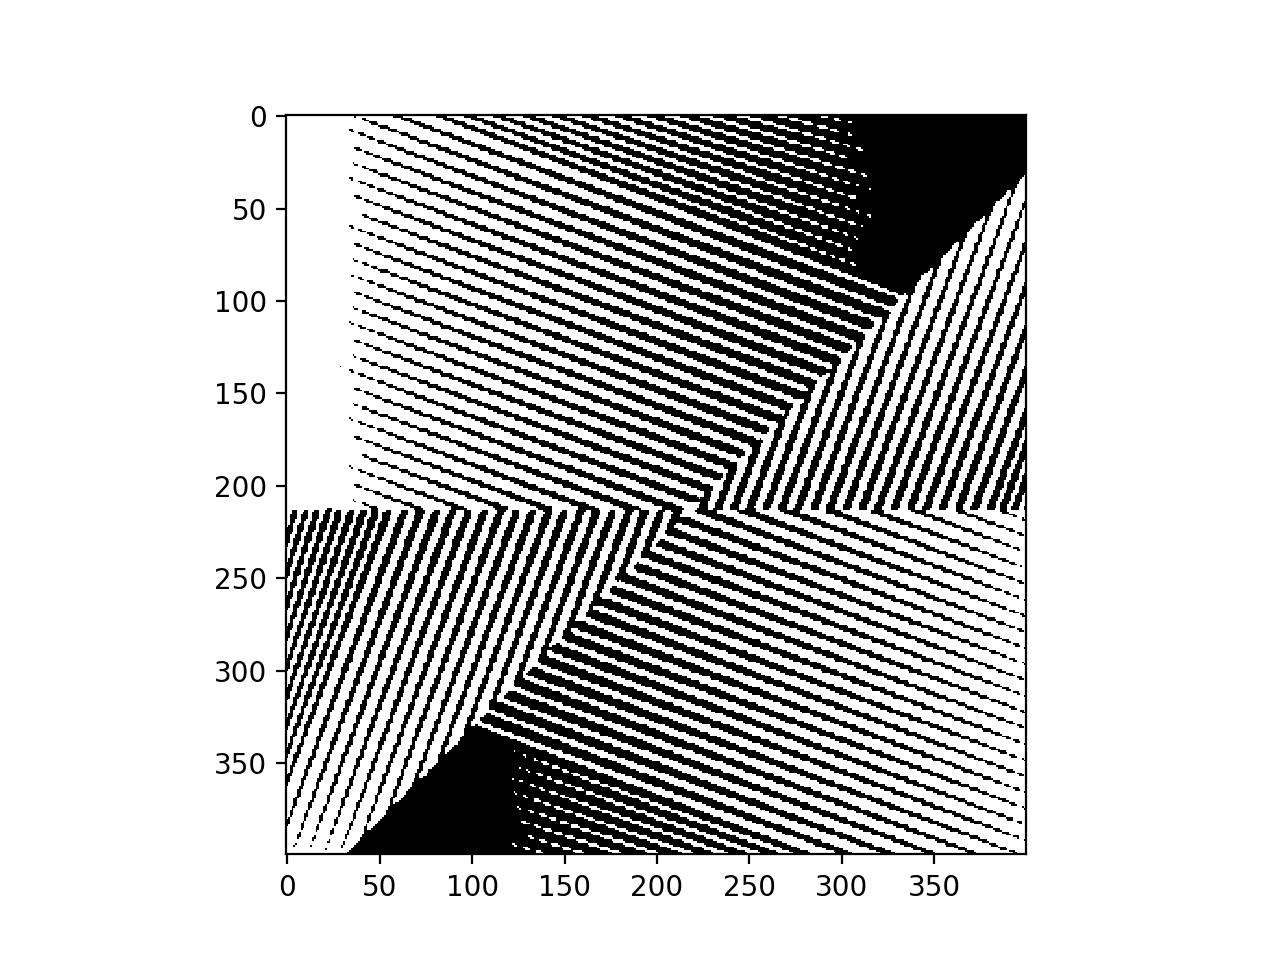
\includegraphics[width=\linewidth]{{fig/E1.6}.png}
  \caption*{Input}
\endminipage\hfill
\minipage{0.25\textwidth}
    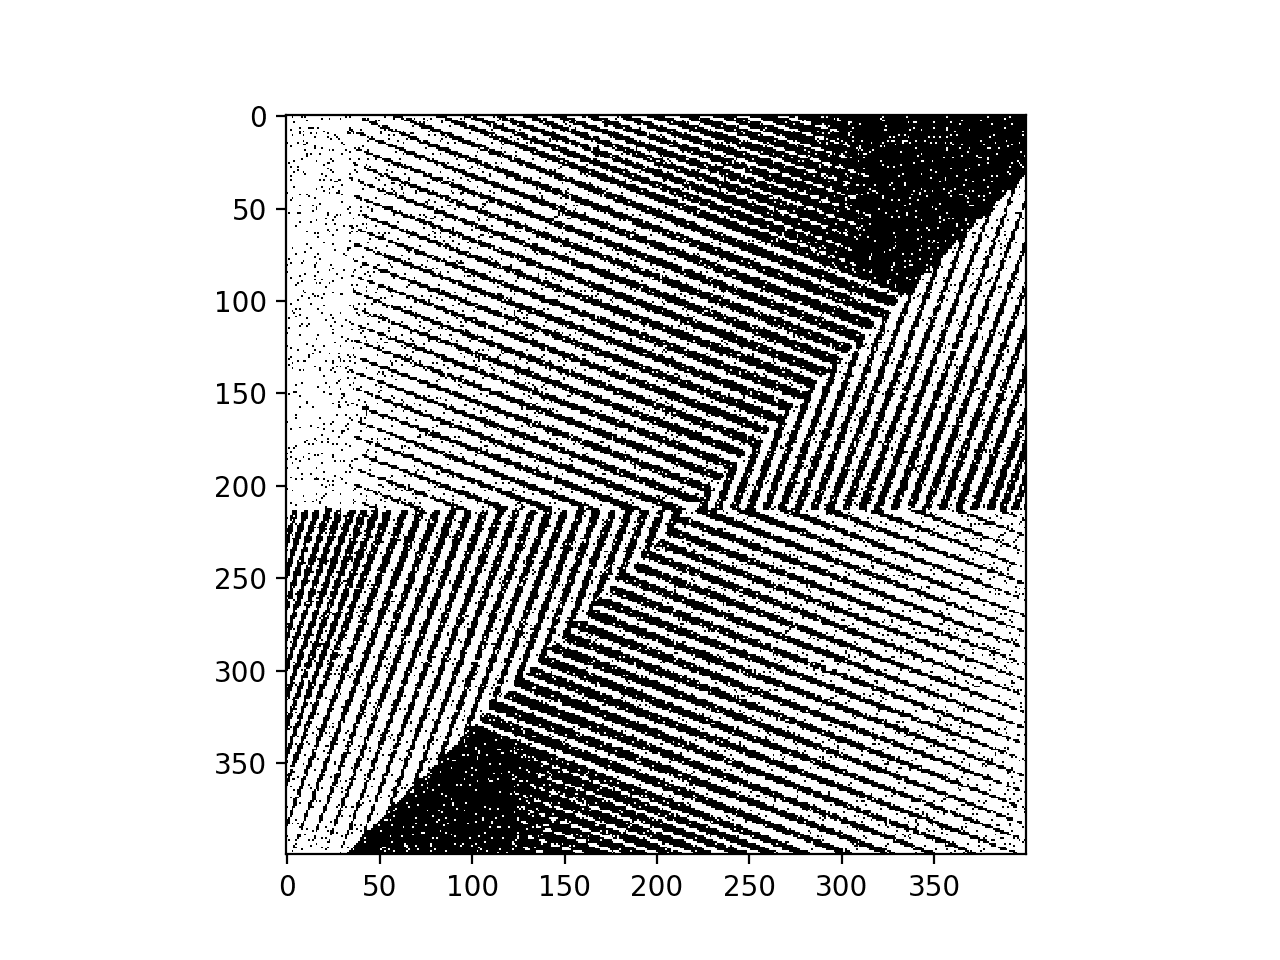
\includegraphics[width=\linewidth]{{fig/E1.6_noised}.png}
    \caption*{Noised}
\endminipage\hfill
\minipage{0.25\textwidth}
    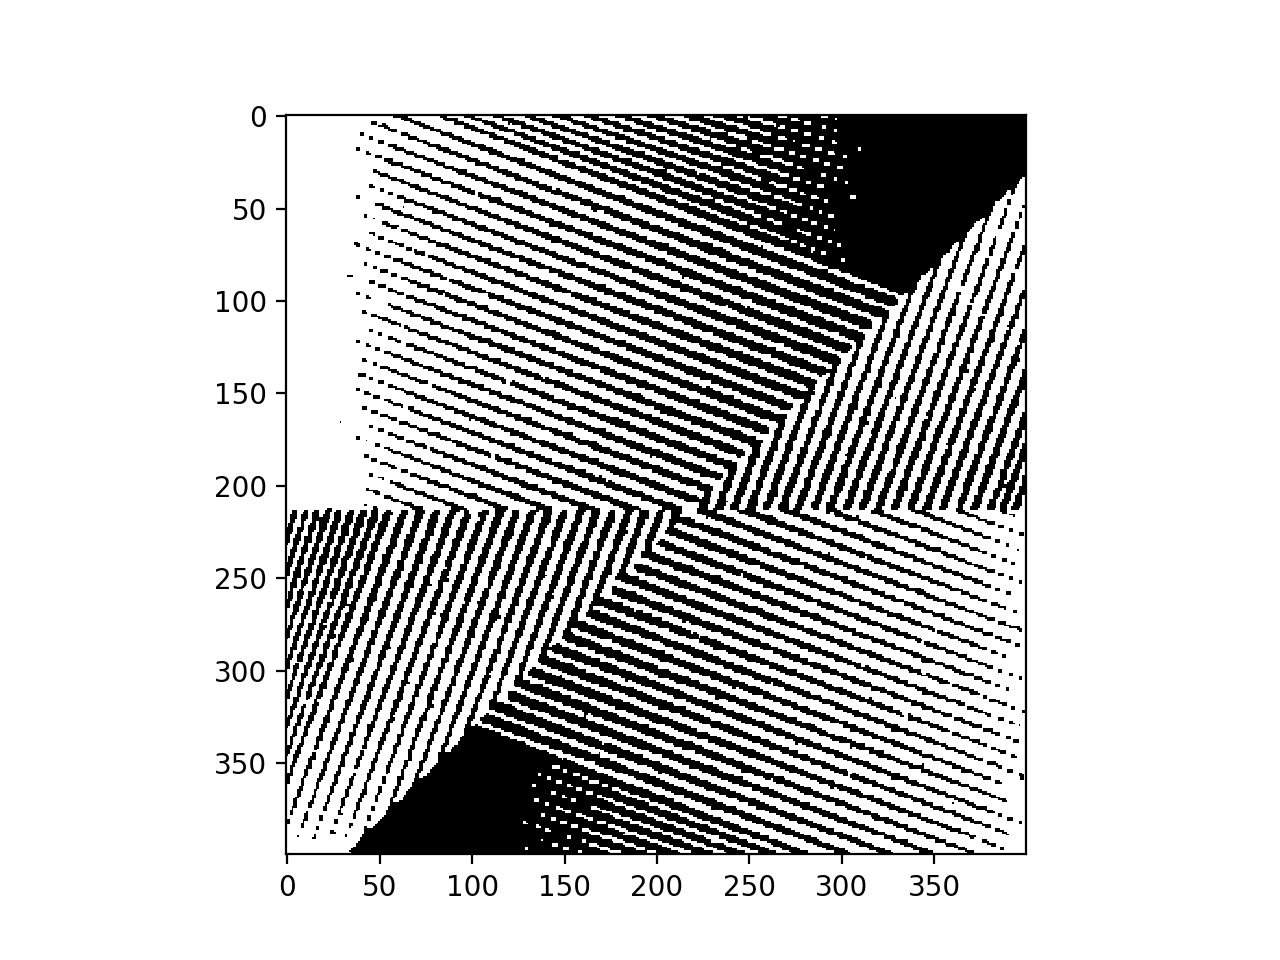
\includegraphics[width=\linewidth]{{fig/E1.6.1}.png}
    \caption*{Original $\Delta E$}
\endminipage\hfill
\minipage{0.25\textwidth}
    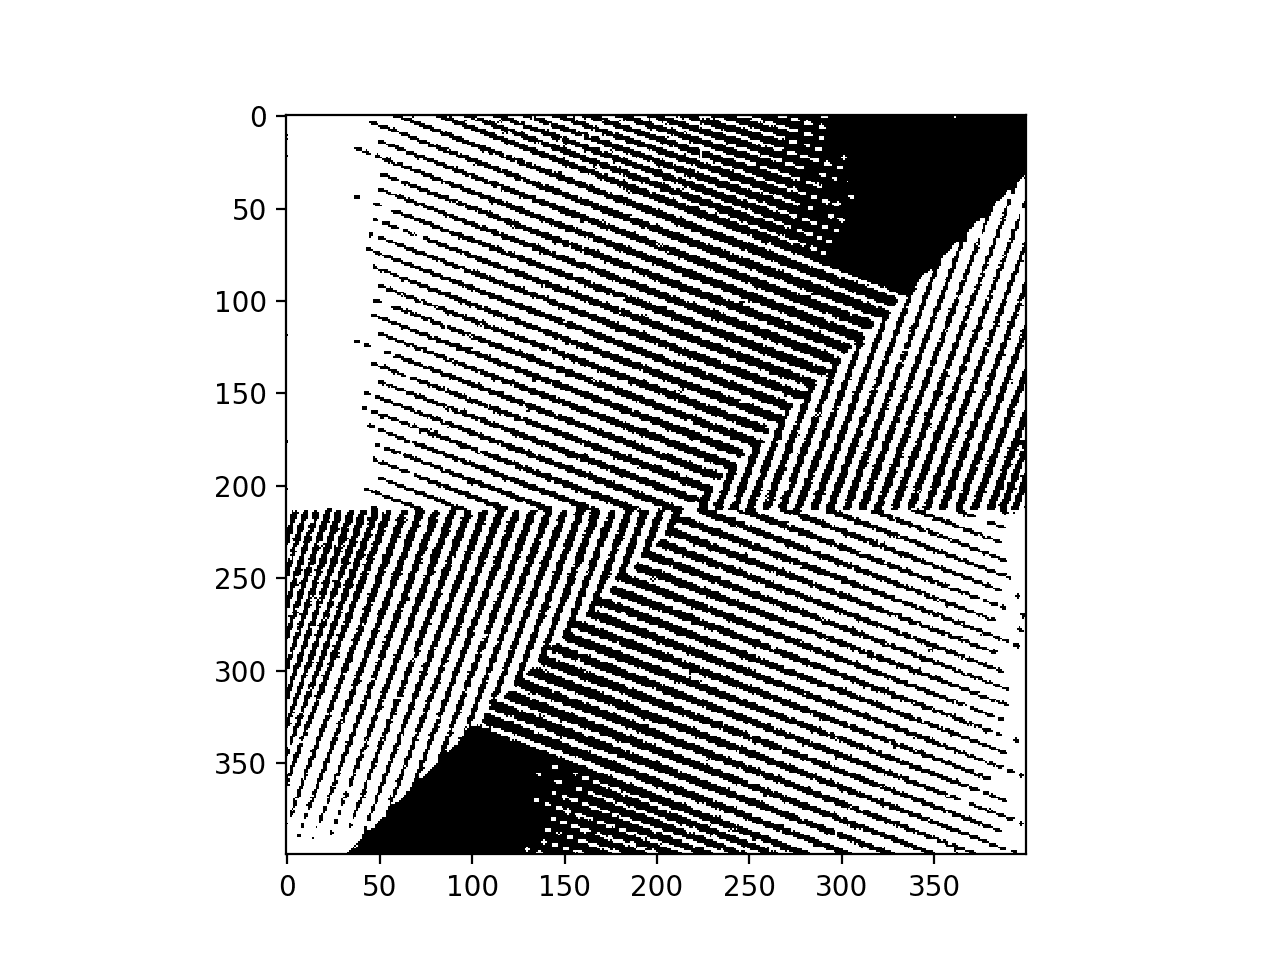
\includegraphics[width=\linewidth]{{fig/E1.6.2}.png}
    \caption*{Updated $\Delta E$}
\endminipage
\end{figure}

This might be a set that is harder to observe the difference. But if you zoom in you will realize the updated $\Delta E$ is more ``connected'' at the end of each edge, which is a better presentation of the original input. This is due to the updated $\Delta E$ takes more and farther nearby pixels into consideration.

\section*{E2. Graphical Representation}

\subsection*{2.1.}

\begin{figure}[H]
    \centering
    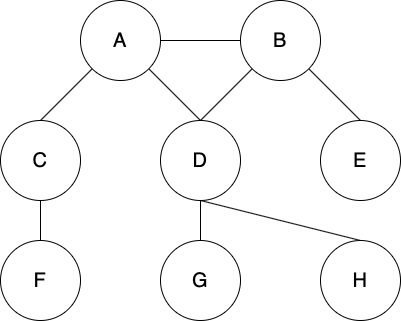
\includegraphics[width=0.3\linewidth]{{fig/E2.1}.png}
\end{figure}

For Bayes net, we have:

\begin{equation*}
    p(a, b, c, d, e, f, g) = p(a)p(b)p(c \mid a)p(d \mid a, b)p(e \mid b)p(f \mid c)p(g \mid d)p(h \mid d)
\end{equation*}

\noindent For MRF, we connect the parents and have:
\begin{equation*}
    p(a, b, c, d, e, f, g) = \psi(a, c)\psi(a, b, d)\psi(b, e)\psi(c, f)\psi(d, g)\psi(d, h)
\end{equation*}
\subsection*{2.2.}

\begin{figure}[H]
    \centering
    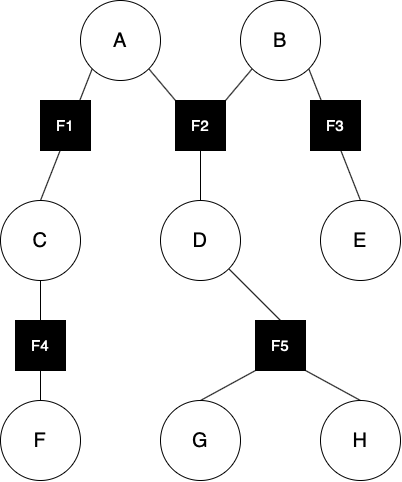
\includegraphics[width=0.3\linewidth]{{fig/E2.2}.png}
\end{figure}

THe joint distribution will be:

\begin{equation*}
    p(a, b, c, d, e, f, g) = f_1(a, c)f_2(a, b, d)f_3(b, e)f_4(c, f)f_5(d, g, h)
\end{equation*}

\subsection*{2.3.}



\begin{figure}[H]
\minipage{0.3\textwidth}
  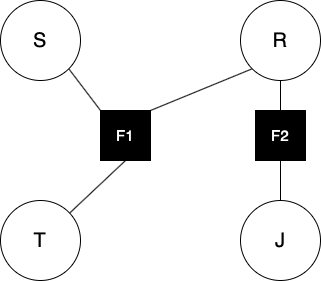
\includegraphics[width=\linewidth]{{fig/E2.3.1}.png}
  \caption*{Graph 1}
\endminipage\hfill
\minipage{0.3\textwidth}
    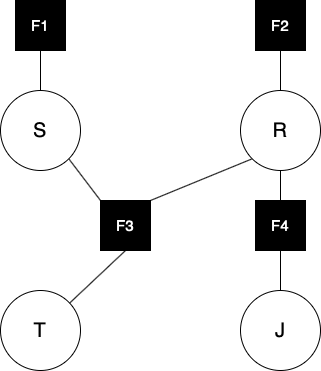
\includegraphics[width=\linewidth]{{fig/E2.3.2}.png}
    \caption*{Graph 2}
\endminipage
\end{figure}

For \textbf{Graph 1}, we added factor functions between all connections, and the probablity function will be:

\begin{align*}
    f_1(S, R, T) &= p(T \mid S, R)p(S)p(R) \\
    f_2(R, J) &= p(J \mid R) \\
    p(S, R, T, J) &= f_1(S, R, T)f_2(R, J) = p(T \mid S, R)p(S)p(R)p(J \mid R)
\end{align*}

On ther other hand for \textbf{Graph 2} we added factor functions for every nodes, thus:

\begin{align*}
    f_1(S) &= p(S) \\
    f_2(R) &= p(R) \\
    f_3(S, R, T) &= p(T \mid S, R) \\
    f_4(R, J) &= p(J \mid R) \\
    p(S, R, T, J) &= f_1(S)f_2(R)f_3(S, R, T)f_4(R, J) = p(S)p(R)p(T \mid S, R)p(J \mid R)
\end{align*}


\section*{E3. The Sum Product Algorithm}

\subsection*{3.1.}

\begin{align*}
    \mu_{a \to f_1} &= \mu_{b \to f_1} = \mu_{d \to f_2} = 1 \\
    \mu_{f_1 \to c} &= \sum_a \sum_b f_1(a, b, c) \mu_{a \to f_1} \mu_{b \to f_1} \\
    \mu_{f_2 \to c} &= \sum_d f_2(c, d)\mu_{d \to f_2}
\end{align*}

\subsection*{3.2.}

\begin{align*}
    p(c) &= \mu_{f_1 \to c}\mu_{f_2 \to c} \\
    &=  \sum_a \sum_b f_1(a, b, c) \mu_{a \to f_1} \mu_{b \to f_1} \cdot \sum_d f_2(c, d)\mu_{d \to f_2} \\
    &= \sum_a \sum_b f_1(a, b, c)  \sum_d f_2(c, d)
\end{align*}

\subsection*{3.3.}

\begin{align*}
    p(c) &= \sum_a \sum_b \sum_d p(a, b, c, d) \\
    &= \sum_a \sum_b \sum_d f_1(a, b, c)  \sum_d f_2(c, d) \\
    &= \sum_a \sum_b f_1(a, b, c)  \sum_d f_2(c, d)
\end{align*}

\subsection*{3.4.}

% \begin{align*}
%     p(c) &= \Pi_{s \in ne(c)} \mu_{f_s \to c} \\
%     &= \mu_{f_1 \to c}\mu_{f_2 \to c} \\
%     &= \sum_a \sum_b f_1(a, b, c) \mu_{a \to f_1} \mu_{b \to f_1} \cdot \sum_d f_2(c, d)\mu_{d \to f_2} \\
%     &= \sum_a \sum_b f_1(a, b, c)  \sum_d f_2(c, d)
% \end{align*}

The information passing of graph-in-question is defined as:

\begin{align*}
    \mu_{a \to f_1} &= \mu_{d \to f_2} = 1 \\
    \mu_{b \to f_1} &= \mu_{f_2 \to b} \\
    \mu_{b \to f_2} &= \mu_{f_1 \to b} \\
    \mu_{f_1 \to b} &= \sum_a \sum_c f_1(a, b, c) \mu_{a \to f_1} \mu_{c \to f_1} \\
    \mu_{f_1 \to c} &= \sum_a \sum_b f_1(a, b, c) \mu_{a \to f_1} \mu_{b \to f_1} \\
    \mu_{f_2 \to b} &= \sum_c \sum_d f_2(b, c, d) \mu_{c \to f_2} \mu_{d \to f_2} \\
    \mu_{f_2 \to c} &= \sum_b \sum_d f_2(b, c, d) \mu_{b \to f_2} \mu_{d \to f_2}
\end{align*}

Now we have:

\begin{align*}
    p(c) &= \mu_{f_1 \to c} \mu_{f_2 \to c} \\
    &= \sum_a \sum_b f_1(a, b, c) \mu_{a \to f_1} \mu_{b \to f_1} \cdot \sum_b \sum_d f_2(b, c, d) \mu_{b \to f_2} \mu_{d \to f_2} \\
    &= \sum_a \sum_b f_1(a, b, c) \mu_{a \to f_1} \mu_{f_2 \to b} \cdot \sum_b \sum_d f_2(b, c, d) \mu_{d \to f_2} \mu_{f_1 \to b}   \\
    &=  \sum_a \sum_b f_1(a, b, c) \mu_{a \to f_1} \sum_c \sum_d f_2(b, c, d) \mu_{c \to f_2} \mu_{d \to f_2} \cdot \sum_b \sum_d f_2(b, c, d) \mu_{d \to f_2} \sum_a \sum_c f_1(a, b, c) \mu_{a \to f_1} \mu_{c \to f_1} \\
    &=  \sum_a \sum_b f_1(a, b, c) \sum_c \sum_d f_2(b, c, d) \mu_{c \to f_2} \cdot \sum_b \sum_d f_2(b, c, d)  \sum_a \sum_c f_1(a, b, c) \mu_{c \to f_1}\\
    &= \sum_a \sum_b f_1(a, b, c)  \mu_{f_2 \to b} \cdot \sum_b \sum_d f_2(b, c, d) \mu_{f_1 \to b} \\
    &...
\end{align*}

The equation will eventually include itself and therefore become an infinite loop.

\section*{Exploration}

For this exploration I'd like to explore more about image denoising. I will first talk about my experience with \textit{image stacking}, a popular image denoising method used by modern photographer. Then I will discuss paper \href{https://arxiv.org/abs/1901.06046}{Good Similar Patches for Image Denoising} by Lu.\newline

\noindent My dad and I are both photographers, and I was lucky enough to have an early and healthy exposure to many photography gears and concepts. Ever since I was semi-fluent on computers, Photoshop become one of my favourite thing to study on; and I have spent much of my middle/highschool life reading random tutorials online to learn a new ``trick'' or two. And one day I came across the concept of \textit{image stacking}, although I haven't realized much back then, that might be my first ``relatively in-depth'' experience to image denoising.


Modern landscape photography tends to push cameras into their limits, mostly because of the popularity of taking images with high dynamic range -- which can be roughly understood as the brightness difference between the lightest and the darkest pixel within the same image. Because image with high dynamic range are friendly to post-processing and the retouched version of such images may have the ``HDR-like'' affect that is very catchy to audiances (we typically can't capture such large range of brightness at the same time with raw eyes).

\begin{figure}[H]
    \centering
    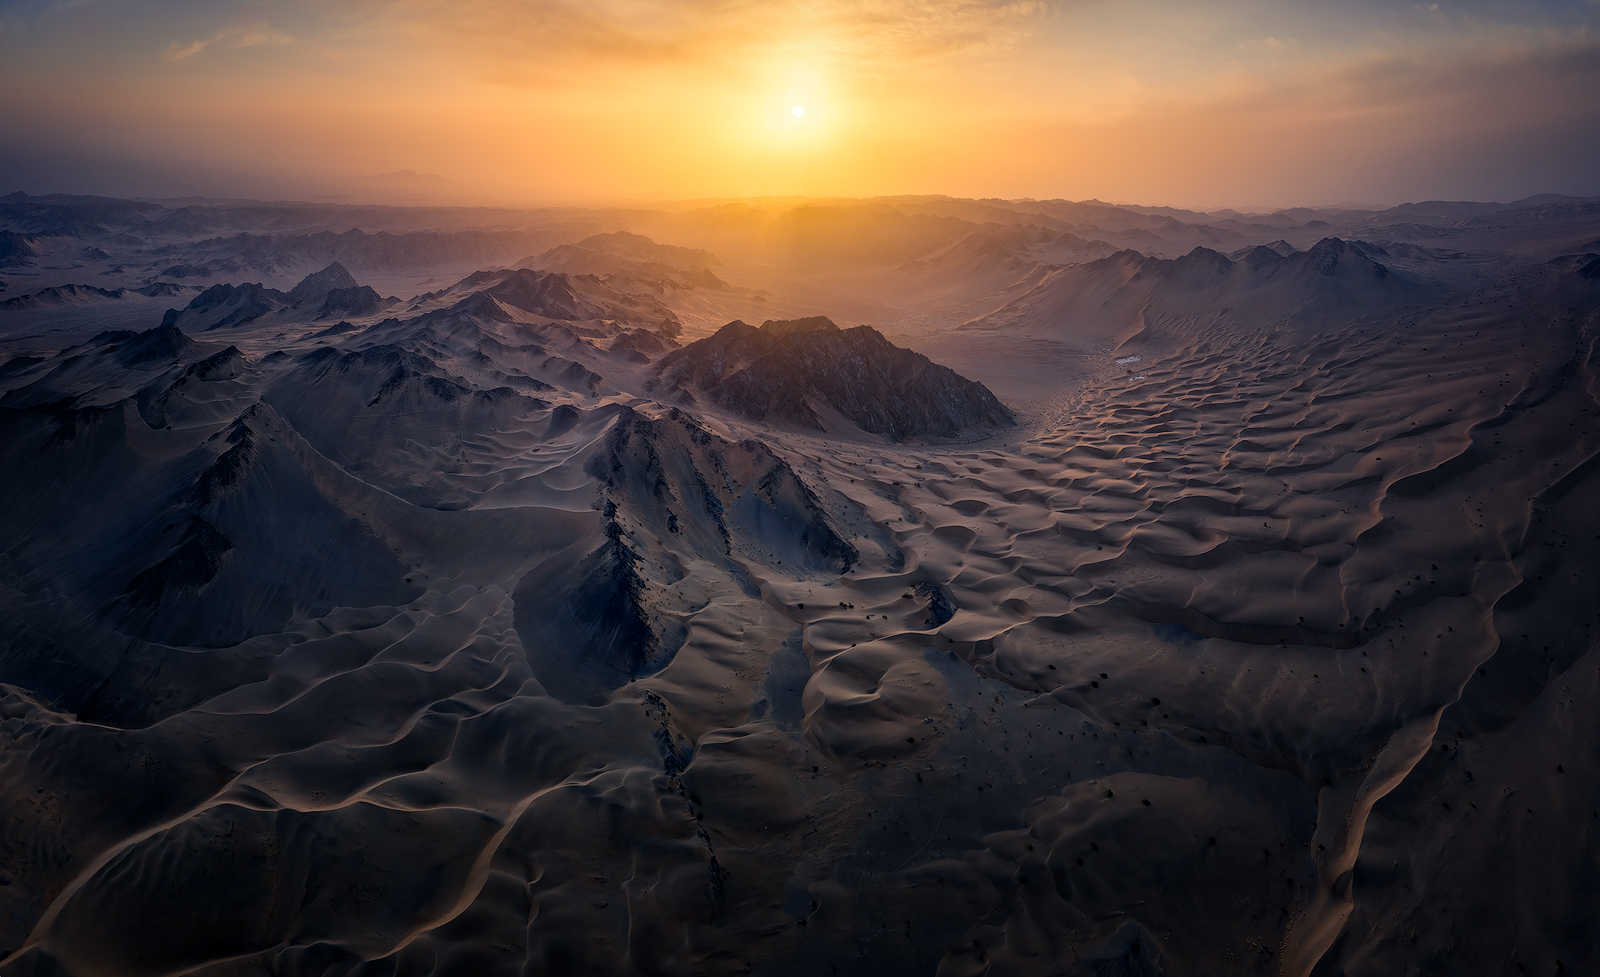
\includegraphics[width=1\linewidth]{{fig/E3.1}.jpg}
    \caption*{The Dunhuang frescoes, by Thomas Chu}
\end{figure}


However, high dynamic range photography has one intrinsic problem to solve: the darker side of the image are often ``under exposure'' and therefore prone to noises and information losing. And there are three typical solutions to this problem: ND filters, HDR, or image stacking. The first two are essentially the same solution, as we simply ``lighten up'' the darker side of the image to gain more information.

\begin{figure}[H]
    \centering
    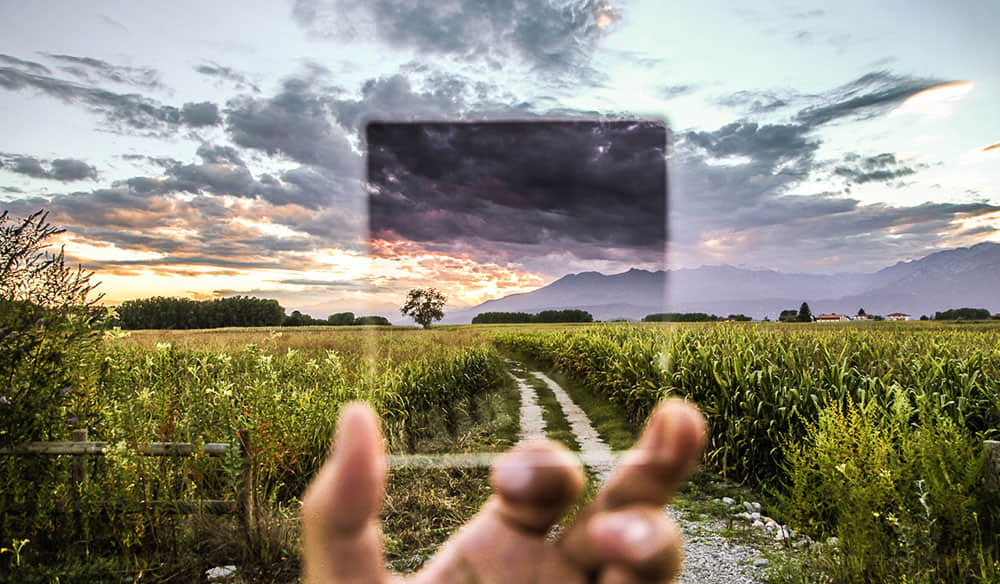
\includegraphics[width=0.5\linewidth]{{fig/E3.2}.jpg}
    \caption*{ND Filter demo}
\end{figure}

With the difference being ND filter does it with one-take, but HDR requires multiple exposures (with different light flux setting, usually controlled by shutter speed) and combining multiple images into one in post processing. We may say the apporach of these two methods is to proactively eliminate noise to find the \textit{ground truth} version of photo. But sometime these two methods are infesible, e.g., the brightness difference (\textit{stops}) of your ND filter is not high or sutiable enough for the scene, there are moving object in the scene so you can't easily combine two images together or the noise is still high after such approach, etc. And image stacking may come at your rescue.\newline

The difficulty of real word image denoising task is there is no \textit{ground truth} of a photo. As every photo you took contain a certain amount of noise, and there's no way you can idealy quantify the noisy-level of an image. So the philosophy of image stacking is simply do ``repetition,'' where you record the same scene with the same setting for a large amount of times. As (a portion of) noise are essentially randomly captured, with repetition, we may identify the noisy-pixels and patch them with pixels from other images. This brings superior performance, as you can always push for higher SNR with more repetition and you got mutiple chance to identify a noise and select patches. It is also friendly to moving objects, as you got a continuous series of images to ``blur it out'' and pratically, it is easy to execuate by leaving your camera on a tripod and wait.


\begin{figure}[H]
    \centering
    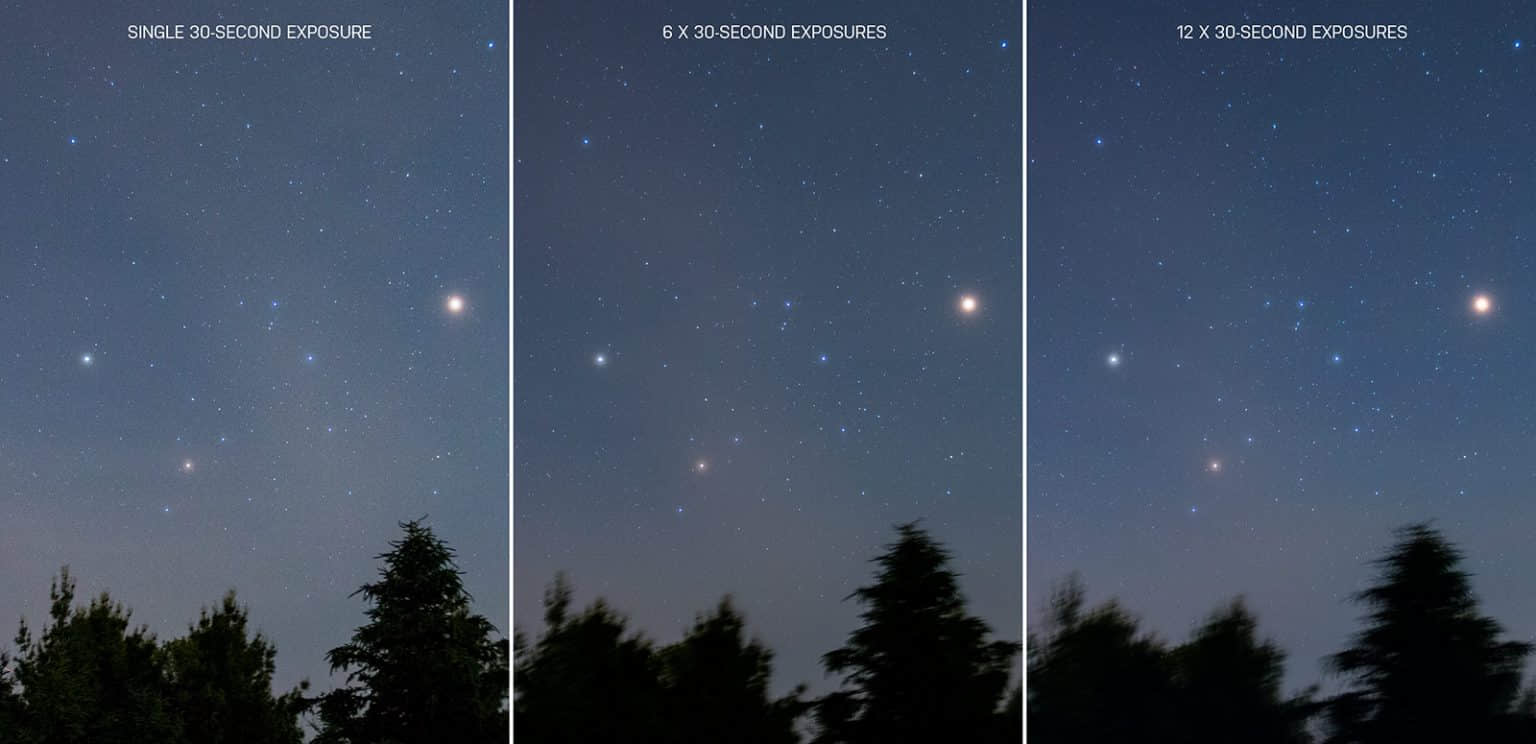
\includegraphics[width=1\linewidth]{{fig/E3.3}.jpg}
    \caption*{Image Stacking demo, visible improvement on the RHS with more images being stacked}
\end{figure}

\noindent So image stacking is an effective method because it can easily identify the noisy-pixel, which will be the most deviated pixel among the stack (on the same coordiate); and it is straighforward on finding patch, as it will be the average of pixel which we deemed to be not noise. In \textbf{Exercise 1} of this assignment, we only focused on identifying noise due to the nature of the input image is binary. But in real word application, noise are often relatively easy to identify -- as you can easily recognize a chroma noise out of an image -- but what to patch the noise with, is often regarded as a harder question to answer.

In this assignment, we center our patch searching as the noisy-pixel, where we evaluate the neighbors of the noisy-pixel to determine the patch -- this is regarded as \textit{Nearest Neighbour Search (NNS)}. However, in non-binary setting, the neighbors of a noisy-pixel may (and often are) under influence of other noise, and therefore renders a patch which is far from the ground truth of the image.

\begin{figure}[H]
    \centering
    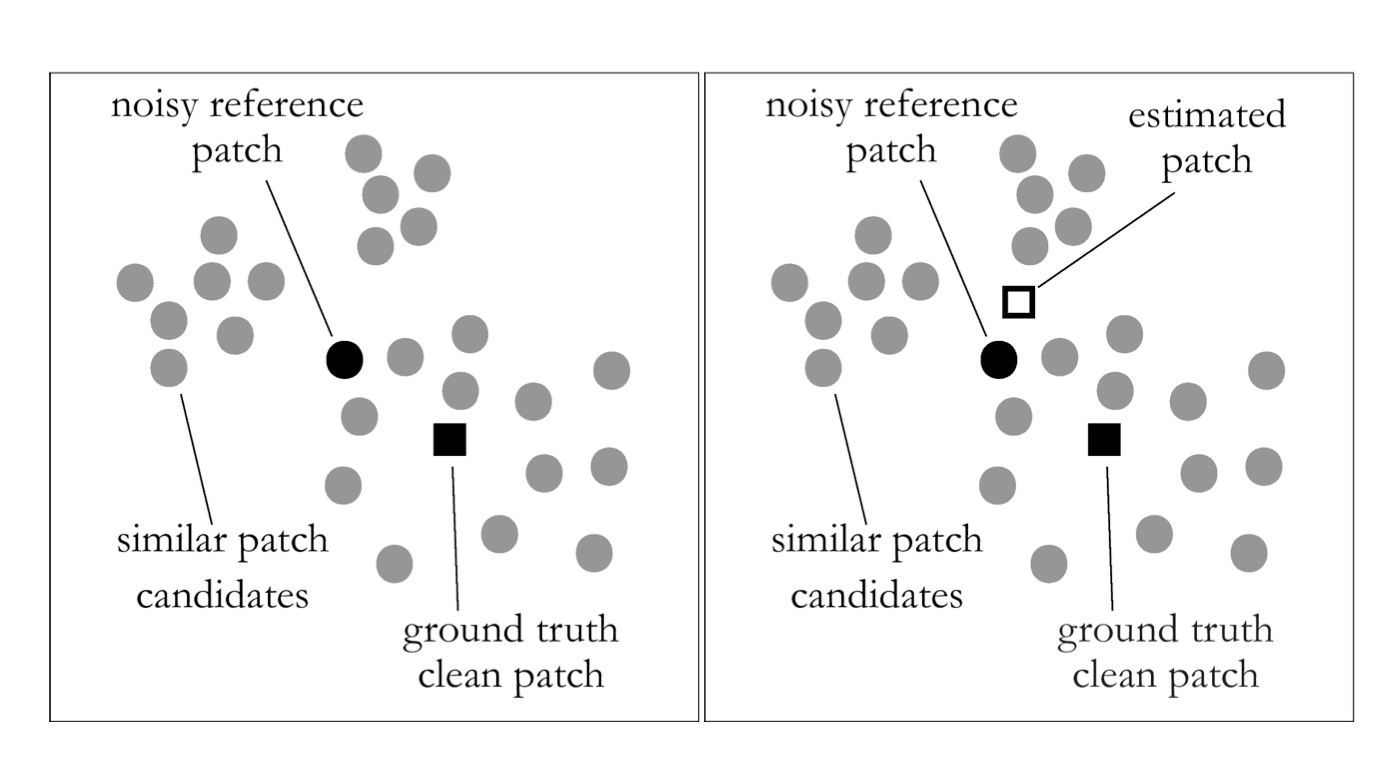
\includegraphics[width=0.6\linewidth]{{fig/E3.4}.png}
    \caption*{In this case, the NNS candidate (blank square) to the noisy black circle is far away from the ground truth patch (black square)}
\end{figure}

To address this problem, Lu proposed a method to select patch by conduct clustering on candidate patch groups.

\begin{figure}[H]
    \centering
    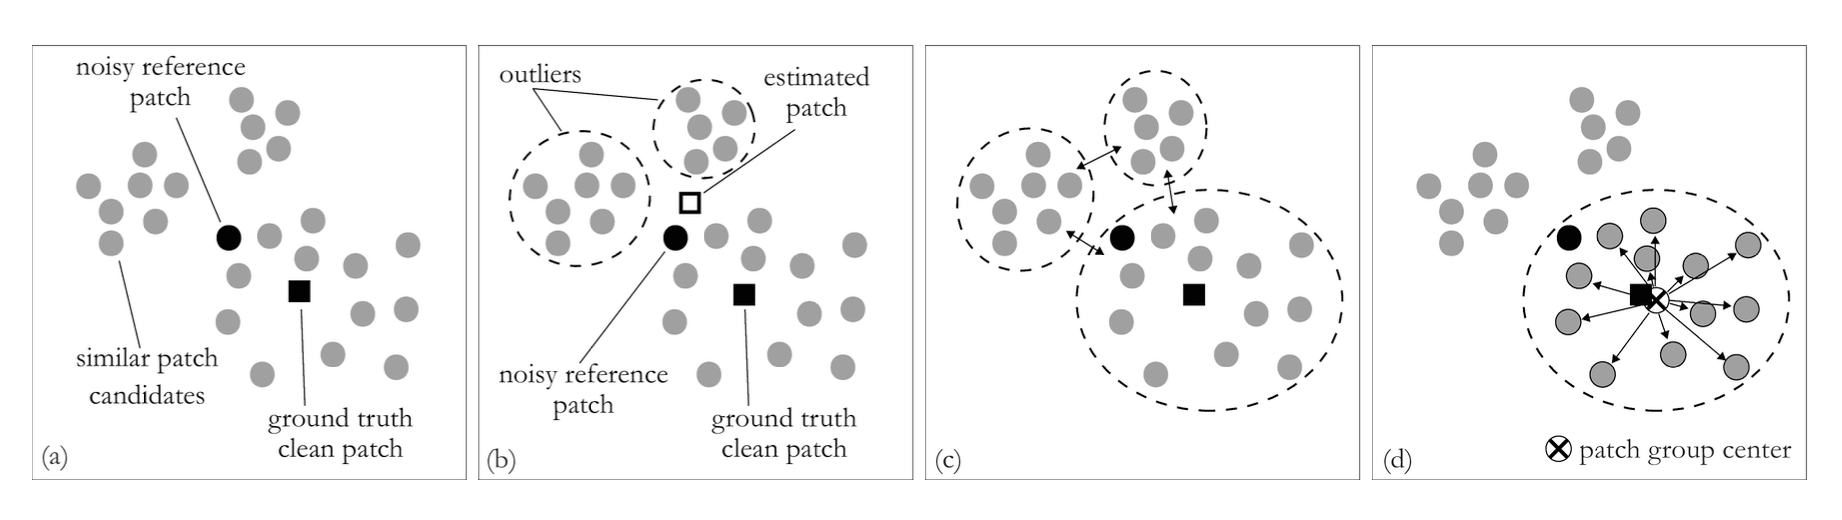
\includegraphics[width=1\linewidth]{{fig/E3.5}.png}
    \caption*{Lu's method of patch selection}
\end{figure}

The takeaway of Lu's approach is to not to center the path search among the noisy reference, but to cluster all nearby pixels into different patch groups first. Then measure the distance between the noisy reference to center of different patch groups, and select patch from the patch group with closest distance.

Lu introduced that each patch group can be modeled as a Gaussian function, and the whole set of candidate patches can be approximated as a Gaussian Mixture Model. The clustering will follow the the Minimum Decription Length criteria:

\begin{equation*}
    MDL (K, \theta) = - \log p_{Q}(Q \mid K, \theta) + \lambda L \log(mn)
\end{equation*}

The first term is defined as:

\begin{equation*}
    - \log p_{Q}(Q \mid K, \theta) = \sum_{k = 1}^K \sum_{j = 1}^{m_k} || q_j - u_k ||^2
\end{equation*}

% L &= K(1 + n + \frac{(n +1)n}{2}) - 1
where $m_k$ and $\mu_k$ are the number of patches in the $k$-th cluster and its centroid. Since the goal is to minimize the $MDL (K, \theta)$, clusters with small ``diameter'' and therefore smaller intra-patch distances are prefered. Note here $Q$ is a set of $m$ \ $n-$dimensional candidate patches, and $\theta$ is the paramaters of GMM.

\begin{equation*}
    L = K(1 + n + \frac{(n +1)n}{2}) - 1
\end{equation*}

The author refered the second term of his $MDL (K, \theta)$ equation as a regularization term to punish large clusters, and $\lambda$ to be a paramater that balances the contribution of two terms. Well I don't quite understand why would he make such complicate of a $L$ since $m$ directly defines the size of a cluster; it seems $L$ is doubled as a definition of number of parameters used in $\theta$ (The author also shows with optimization of K-means++ on clustering, the regularization term will be a constant and can be ignored). After all the goal is to have many small clusters (in terms of diameters and sizes), so that we may have more candidate to attribute our noisy reference to. And intuitively, such clustering will be more fine grained and therefore result in better patch selection: the relationship the ground trutch patch and the selected patch will be closer (as they are in a small cluster), and therefore a better patch can be selected if we may attribute the noisy reference to the right cluster. .\newline


The author then go on and optimized his algorithm with \textit{unrelisable pixel detection} algorithm to detect the noisy reference. He further testified his method -- as a plug of many classic patch-based denoising algorithms -- and demonstrated state-of-the-art performance on some typical image denoising dataset. Since this is my only exposure to image denoising paper, I can't offer much insight about its performance in comparision to the others. Judging from the demo images in paper, the improvement does seem significant.

\begin{figure}[H]
    \centering
    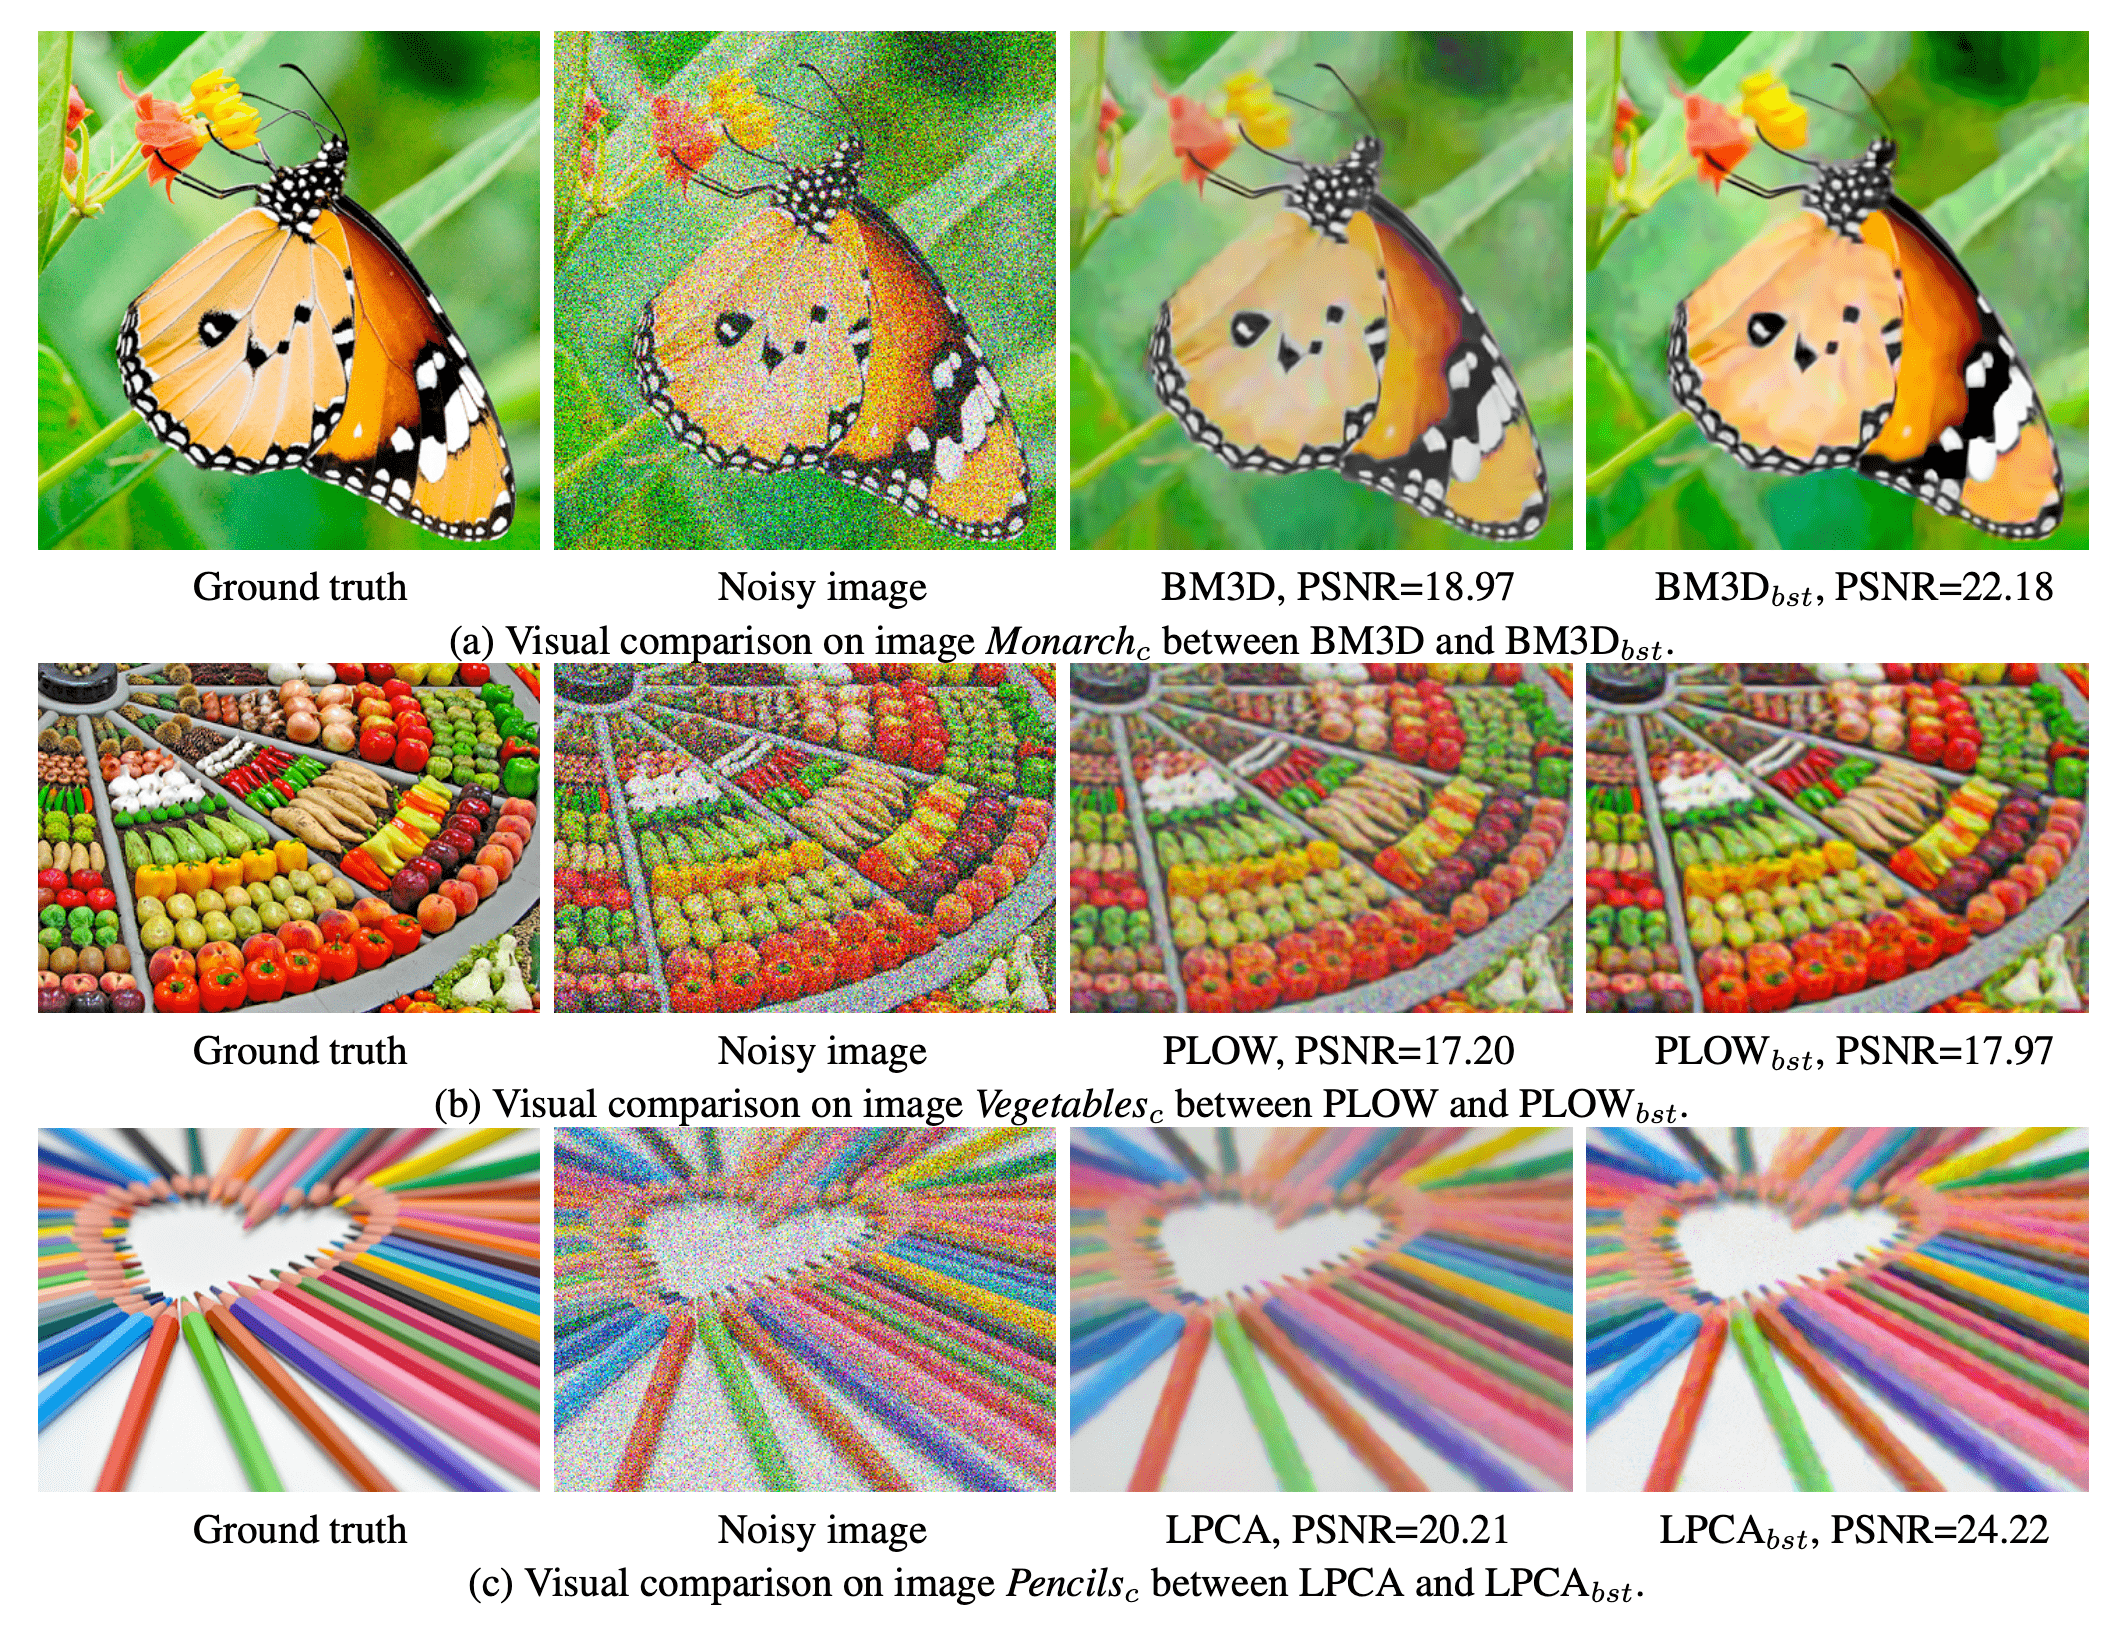
\includegraphics[width=0.7\linewidth]{{fig/E3.6}.png}
    \caption*{\textit{BST} shows improvement on three different denoising algorithms}
\end{figure}

\end{document}

